% -----------------------------------------------------------------------------
%
% Copyright (c) 2017 Sam Cox, Roberto Sommariva
%
% This file is part of the AtChem2 software package.
%
% This file is covered by the MIT license which can be found in the file
% LICENSE.md at the top level of the AtChem2 distribution.
%
% -----------------------------------------------------------------------------

% -------------------- PREAMBLE -------------------- %
\documentclass[11pt,a4paper]{report}
\usepackage{helvet,graphicx,hyperref}
\usepackage{fancyhdr,caption,natbib}
\usepackage[dvipsnames]{xcolor}
\usepackage[version=3]{mhchem}

% page style
\pagestyle{fancy}
\setlength{\headheight}{13.6pt}
\rhead{\leftmark}
\lhead{}

\renewcommand{\bibname}{References}
\frenchspacing

% links
\hypersetup{colorlinks=true,
  linkcolor=BrickRed,
  citecolor=ForestGreen,
  urlcolor=NavyBlue}

% shortcuts
\newcommand{\maindir}{\texttt{\em Main Directory}}
\newcommand{\depdir}{\texttt{\em Dependencies Directory}}
\newcommand{\sharedir}{\texttt{\em Shared Library Directory}}

\newcommand{\degc}{^\circ\mathrm{C}}

% figures
\graphicspath{{../figures/}}

% -------------------- DOCUMENT -------------------- %
\begin{document}

% -------------------------------- %
% Vertical Line Title Page
%
% Template created by P. Wilson, modified by Vel
% https://www.latextemplates.com/template/vertical-line-title-page
%
% License: CC BY-NC-SA 3.0 (https://creativecommons.org/licenses/by-nc-sa/3.0/)

\begin{titlepage}
  \raggedleft   % Right align the title page
  \rule{1pt}{\textheight}  % Vertical line
  \hspace{0.05\textwidth}
  % Box for the title page text
  \parbox[b]{0.75\textwidth}{
    {\Huge\bfseries AtChem2\\[0.5\baselineskip] v1.3-dev}\\[2\baselineskip]  % Title
    {\LARGE\textit{User Manual}}\\[4\baselineskip]  % Subtitle
    {\Large\textsc{R. Sommariva\\S. Cox}}  % Author(s)
    \vspace{0.5\textheight}\\
    {\noindent \today}\\[\baselineskip]  % Date
    }

\end{titlepage}

% -------------------------------- %

\tableofcontents

% -----------------------------------------------------------------------------
%
% Copyright (c) 2017 Sam Cox, Roberto Sommariva
%
% This file is part of the AtChem2 software package.
%
% This file is covered by the MIT license which can be found in the file
% LICENSE.md at the top level of the AtChem2 distribution.
%
% -----------------------------------------------------------------------------

\chapter{Introduction} \label{ch:introduction}

\textbf{AtChem2} is an open source modelling tool for atmospheric
chemistry.  It is designed to build and run zero-dimensional
box-models using the Master Chemical Mechanism
(\href{http://mcm.leeds.ac.uk/MCM/}{MCM}).  The \textbf{MCM} is a
near-explicit chemical mechanism which describes the gas-phase
oxidation of primary emitted Volatile Organic Compounds (VOC) to
carbon dioxide (\cf{CO2}) and water (\cf{H2O}). The MCM protocol is
detailed in \citet{jenkin_1997} and subsequent updates
\citep{saunders_2003, jenkin_2003, bloss_2005, jenkin_2015}. Although
it is meant to be used with the MCM, AtChem2 can use any other
chemical mechanism, as long as it is in the correct format
(Sect.~\ref{sec:chemical-mechanism}).

AtChem2 is a development of \textbf{AtChem-online}, a modelling web
tool created to facilitate the use of the MCM in the simulation of
laboratory and environmental chamber experiments within the
\href{https://www.eurochamp.org/}{EUROCHAMP} community
\citep{martin_2009}. AtChem-online runs as a web service -- provided
by the University of Leeds --and can be accessed at
\href{https://atchem.leeds.ac.uk/webapp/}{https://atchem.leeds.ac.uk/webapp/}:
in order to use AtChem-online, a user needs only a text editor, file
compression software, a web browser, and an internet connection. A
tutorial -- with examples and exercises -- is available on the MCM
\href{http://mcm.leeds.ac.uk/MCMv3.3.1/atchem/tutorial_intro.htt}{website}.

AtChem-online is easy to use even for inexperienced users but has a
number of limitations, mostly related to its nature as a web
application. AtChem2 was developed from AtChem-online with the
objective to provide an \emph{offline} modelling tool capable of
running long simulations of computationally intensive models, as well
as batch simulations for sensitivity studies. In addition, AtChem2
implements a continuous integration workflow, coupled with a
comprehensive suite of tests and version control software
(\href{https://git-scm.com/}{git}), which makes it robust, reliable
and traceable.

The codebase of AtChem2 is structured into four components (or layers)
-- as illustrated in Fig.~\ref{fig:atchem-arch} -- and is written
mostly in Fortran 90/95.  Installation, compilation and execution of
AtChem2 are semi-automated via a number of shell and Python scripts
that require minimal input from the user. This document
(\texttt{AtChem2-Manual.pdf}) is the AtChem2 user manual and contains
all the information required to install, set up and use the current
version of AtChem2. A summary of these instructions, and additional
information, can be found on the
\href{https://github.com/AtChem/AtChem2/wiki/}{wiki}.

\begin{figure}[htb]
  \centering
  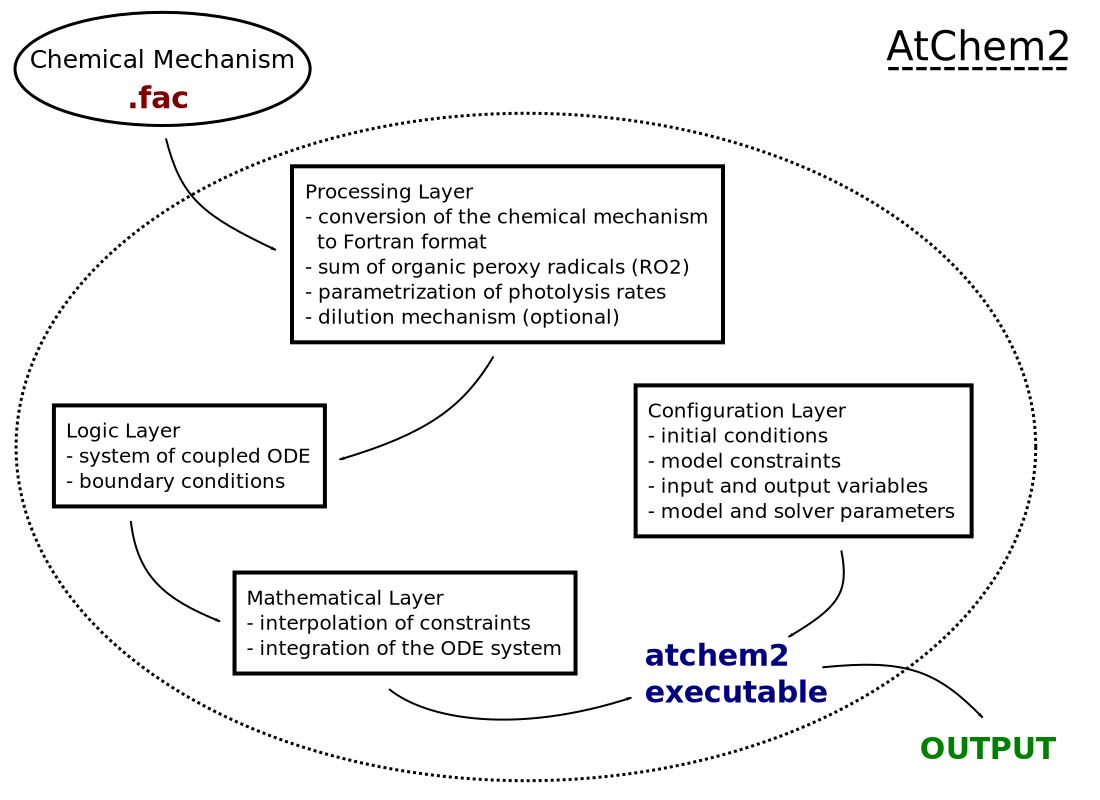
\includegraphics[width=0.8\textwidth]{atchem-structure.png}
  \caption{Architecture of AtChem2.}
  \label{fig:atchem-arch}
\end{figure}

% -------------------------------------------------------------------- %
\section{License and citation} \label{sec:license-citation}

AtChem2 is open source -- released under \textbf{MIT license} -- and is hosted
at \href{https://github.com/AtChem/AtChem2}{https://github.com/AtChem/AtChem2}.
A copy of the license can be found in the \texttt{LICENSE.md} file.

The model is free to use, compatible with the terms of the MIT
license; if used in a publication please include a citation to
the following paper:\\

R.~Sommariva, S.~Cox, C.~Martin, K.~Boro{\'n}ska, J.~Young, P.~K. Jimack,
M.~J. Pilling, V.~N. Matthaios, B.~S. Nelson, M.~J. Newland, M.~Panagi,
W.~J. Bloss, P.~S. Monks, and A.~R. Rickard.
\textbf{AtChem (version 1), an open-source box model for the Master Chemical Mechanism}.
\textit{Geoscientific Model Development}, 13, 1, 169--183, 2020.
doi: \href{https://doi.org/10.5194/gmd-13-169-2020}{10.5194/gmd-13-169-2020}.

% -----------------------------------------------------------------------------
%
% Copyright (c) 2017 Sam Cox, Roberto Sommariva
%
% This file is part of the AtChem2 software package.
%
% This file is covered by the MIT license which can be found in the file
% LICENSE.md at the top level of the AtChem2 distribution.
%
% -----------------------------------------------------------------------------

\chapter{Model Installation} \label{ch:installation}

% -------------------------------------------------------------------- %
\section{Requirements} \label{sec:requirements}

AtChem2 can be installed on Linux/Unix and macOS operating systems. A
working knowledge of the \textbf{unix shell} and its
\href{https://swcarpentry.github.io/shell-novice/reference/}{basic commands}
\emph{is required} to install and use the model. AtChem2 requires the
following tools:

\begin{itemize}
\item Fortran -- the model compiles with GNU \texttt{gfortran} (version
  4.8.5) and with Intel \texttt{ifort} (version 17.0)\\
  \textbf{default compiler}: GNU \texttt{gfortran}
\item Python
\item cmake
\item Ruby (optional)
\end{itemize}

Some or all of these tools may already be present on your operating
system. Use the \texttt{which} command to find out (e.g.:
\verb|which python|, \verb|which cmake|, etc\ldots). Otherwise, check
the local documentation or ask the system administrator. In addition,
AtChem2 has the following dependencies:

\begin{itemize}
\item CVODE
\item openlibm
\item BLAS and LAPACK
\item numdiff (optional)
\item FRUIT (optional)
\end{itemize}

For detailed instructions on the installation and configuration of the
dependencies go to Sect.~\ref{sec:dependencies}.

% -------------------------------------------------------------------- %
\section{Download} \label{sec:download}

There are two versions of AtChem2: the
\href{https://github.com/AtChem/AtChem2/releases}{stable version} and
the development version, also known as \texttt{master\ branch} (see
Chapt.~\ref{ch:development} for additional information). The source
code can be obtained in two ways:

\begin{itemize}
\item with \textbf{git}:
  \begin{enumerate}
  \item Open the terminal. Move to the directory where you want to
    install AtChem2.
  \item Execute \verb|git clone https://github.com/AtChem/AtChem2.git|
    (if using HTTPS) or \verb|git clone git@github.com:AtChem/AtChem2.git|
    (if using SSH). This method will download the development version
    and it is recommended if you want to contribute to the model
    development.
  \end{enumerate}
\item with the \textbf{archive file}:
  \begin{enumerate}
  \item Download the archive file (\texttt{*.tar.gz} or \texttt{*.zip}) of the
    \href{https://github.com/AtChem/AtChem2/releases}{stable version} or of the
    \href{https://github.com/AtChem/AtChem2/archive/master.zip}{development version}
    to the directory where you want to install AtChem2.
  \item Open the terminal. Move to the directory where the archive
    file was downloaded.
  \item Execute \verb|tar -zxfv v1.0.tar.gz| or
    \verb|unzip -v master.zip| (depending on which archive was
    downloaded) to unpack the archive file.
  \end{enumerate}
\end{itemize}

The AtChem2 source code is now in a directory called \texttt{AtChem2}
(if git was used) or \texttt{AtChem2-1.0}  
(if the stable version was
downloaded) or \texttt{AtChem2-master} (if the development version was
downloaded). This directory, which can be given any name, is the
\maindir\ of the model. In this manual, the \maindir\ is assumed to
be: \texttt{\$HOME/AtChem2}.

% -------------------------------------------------------------------- %
\section{Dependencies} \label{sec:dependencies}

AtChem2 has a number of dependencies (external tools and libraries):
some are required, and without them the model cannot be installed or
used, others are optional. It is recommended to use the same directory
for all the dependencies of AtChem2: the \depdir\ can be located
anywhere and given any name. In this manual, the \depdir\ is
assumed to be: \texttt{\$HOME/atchem-lib/}.

Before installing the dependencies, make sure that a \textbf{Fortran}
compiler, \textbf{Python}, \textbf{cmake} and (optionally)
\textbf{Ruby} are installed on the operating system, as explained in
Sect.~\ref{sec:requirements}.

\subsection{Required dependencies} \label{subsec:required-dependencies}

\subsubsection{BLAS and LAPACK}

BLAS and LAPACK are standard Fortran libraries for linear
algebra. They are needed to install and compile the CVODE library (see
below). Usually they are located in the \texttt{/usr/lib/} directory
(e.g., \texttt{/usr/lib/libblas/} and \texttt{/usr/lib/lapack/}). The
location may be different, especially if you are using a High
Performance Computing (HPC) system: check the local documentation or
ask the system administrator.

\subsubsection{CVODE}

AtChem2 uses the CVODE library which is part of the open source
\href{https://computation.llnl.gov/projects/sundials}{SUNDIALS} suite
\citep{hindmarsh_2005}, to solve the system of ordinary differential
equations (ODE).

The version of CVODE currently used in AtChem2 is v2.9.0 (part of
SUNDIALS v2.7.0) and it can be installed using the \texttt{install\_cvode.sh}
script in the \texttt{tools/install/} directory.

\begin{enumerate}
\item Open the terminal. Move to the \maindir\ (\verb|cd ~/AtChem2|).
\item Open the installation script (\texttt{tools/install/install\_cvode.sh})
  with a text editor:
  \begin{itemize}
  \item If LAPACK and BLAS are not in the default location (see
    above), change the \texttt{LAPACK\_LIBS} variable for your
    architecture (Linux or macOS) as appropriate.
  \item If you are not using the \texttt{gcc} compiler
    (\texttt{gfortran}), change the line
    \texttt{-DCMAKE\_C\_COMPILER:FILEPATH=gcc \textbackslash}
    accordingly.
  \end{itemize}
\item Run the installation script (change the path to the \depdir\ as
  needed):
  \begin{verbatim}
  ./tools/install/install_cvode.sh ~/atchem-lib/
  \end{verbatim}
\end{enumerate}

If the installation is successful, there should be a working CVODE
installation at \texttt{\textasciitilde/atchem-lib/cvode/}. Take note
of the path to the CVODE library (\texttt{\textasciitilde/atchem-lib/cvode/lib/}),
as it will be needed later to complete the configuration of AtChem2
(Sect.~\ref{sec:install}).

\subsubsection{openlibm}

openlibm is a \href{https://openlibm.org/}{portable version} of the
open source libm library. Installing openlibm and linking against it
allows reproducible results by ensuring the same implementation of
several mathematical functions across platforms.

The current version of openlibm is 0.4.1 and it can be installed using
the \texttt{install\_openlibm.sh} script in the \texttt{tools/install/}
directory.

\begin{enumerate}
\item Open the terminal. Move to the \maindir\ (\verb|cd ~/AtChem2|).
\item Run the installation script (change the path to the \depdir\ as
  needed):
  \begin{verbatim}
  ./tools/install/install_openlibm.sh ~/atchem-lib/
  \end{verbatim}
\end{enumerate}

If the installation is successful, there should be a working openlibm
installation at \texttt{\textasciitilde/atchem-lib/openlibm-0.4.1/}.
Take note of the path to openlibm, as it will be needed later to
complete the configuration of AtChem2 (Sect.~\ref{sec:install}).

\subsection{Optional dependencies} \label{subsec:optional-dependencies}

\subsubsection{numdiff}

numdiff is a \href{https://www.nongnu.org/numdiff/}{program} used to
compare files containing numerical fields. It is needed only if you
want to run the \hyperref[sec:test-suite]{Test Suite}, a series of
tests used to ensure that the model works properly and that changes to
the code do not result in unintended behaviour. Installation of
numdiff is recommended if you want to contribute to the development of
AtChem2.

Use \verb|which numdiff| to check if the program is already installed
on your system. If not, ask the system administrator. Alternatively,
numdiff can be installed locally (e.g., in the \depdir) using the
script \texttt{install\_numdiff.sh} in the \texttt{tools/install/}
directory.

\begin{enumerate}
\item Open the terminal. Move to the \maindir\ (\verb|cd ~/AtChem2|).
\item Run the installation script (change the path to the \depdir\ as
  needed):
  \begin{verbatim}
  ./tools/install/install_numdiff.sh ~/atchem-lib/
  \end{verbatim}
\item Move to the \texttt{\$HOME} directory (\texttt{cd\ \textasciitilde}).
  Open the \texttt{.bash\_profile} file (or the \texttt{.profile}
  file, depending on your configuration) with a text editor. Add the
  following line to the bottom of the file (change the path to the
  \depdir\ as needed):
  \begin{verbatim}
  PATH=$PATH:$HOME/atchem-lib/numdiff/bin
  \end{verbatim}
\item Close the terminal.
\item Reopen the terminal. Execute \verb|which numdiff| to check that
  the program has been installed correctly.
\end{enumerate}

\subsubsection{FRUIT}

FRUIT (FORTRAN Unit Test Framework) is a
\href{https://en.wikipedia.org/wiki/Unit_testing}{unit test framework}
for Fortran. It requires Ruby and it is needed only if you want to run
the unit tests (Sect.~\ref{sec:test-suite}). Installation of FRUIT is
recommended if you want to contribute to the development of AtChem2.

The current version of FRUIT is 3.4.3 and it can be installed using
the \texttt{install\_fruit.sh} script in the \texttt{tools/install/}
directory.

\begin{enumerate}
\item Open the terminal. Move to the \texttt{\$HOME} directory
  (\texttt{cd\ \textasciitilde}). Open the \texttt{.bash\_profile}
  file (or the \texttt{.profile} file, depending on your
  configuration) with a text editor. Add the following lines to the
  bottom of the file:
  \begin{verbatim}
  GEM_HOME=$HOME/.gem
  PATH=$PATH:$GEM_HOME/bin
  \end{verbatim}
\item Close the terminal.
\item Reopen the terminal. Move to the \maindir\ (\verb|cd ~/AtChem2|).
\item Run the installation script (change the path to the \depdir\ as
  needed):
  \begin{verbatim}
  ./tools/install/install_fruit.sh ~/atchem-lib/
  \end{verbatim}
\end{enumerate}

If the installation is successful, there should be a working FRUIT
installation at \texttt{\textasciitilde/atchem-lib/fruit\_3.4.3/}.
Take note of the path to FRUIT, as it will be needed later to complete
the configuration of AtChem2 (Sect.~\ref{sec:install}).


% -------------------------------------------------------------------- %
\section{Install} \label{sec:install}

To install AtChem2:

\begin{enumerate}
\item Open the terminal. Move to the \maindir\ (\verb|cd ~/AtChem2|).
  Install the \hyperref[sec:dependencies]{Dependencies} and take note
  of the names and paths of CVODE, openlibm and FRUIT.
\item Copy the example \texttt{Makefile} from the
  \texttt{tools/install/} directory to the \maindir:
  \begin{verbatim}
  cp ./tools/install/Makefile.skel ./Makefile
  \end{verbatim}
\item Open the \texttt{Makefile} with a text editor. Set the variables
  \texttt{\$CVODELIB}, \texttt{\$OPENLIBMDIR}, \texttt{\$FRUITDIR} to
  the paths of CVODE, openlibm and FRUIT, respectively. Use full
  paths, because using relative paths may cause compilation
  errors~\footnote{See issue
    \href{https://github.com/AtChem/AtChem2/issues/364}{\#364}}.  For
  example (change the path to the \depdir\ as needed):
  \begin{verbatim}
  CVODELIB = $(HOME)/atchem-lib/cvode/lib
  OPENLIBMDIR = $(HOME)/atchem-lib/openlibm-0.4.1
  FRUITDIR = $(HOME)/atchem-lib/fruit_3.4.3
  \end{verbatim}
  If FRUIT has not been installed (it is optional), leave the default
  value for \texttt{\$FRUITDIR}.
\item Compile AtChem2 with the \texttt{build\_atchem2.sh} script in
  the \texttt{build/} directory:
  \begin{verbatim}
  ./build/build_atchem2.sh ./mcm/mechanism_test.fac
  \end{verbatim}
  This command compiles the model and creates an executable (called
  \texttt{atchem2}) using the example mechanism file
  \texttt{mechanism\_test.fac} included in the \texttt{mcm/}
  directory.
\item Execute \verb|./atchem2| from the \maindir\. This command runs
  the model executable using the default configuration. If the model
  run completes successfully, a message similar to this will be
  printed to the terminal:
  \begin{verbatim}
  ------------------
   Final statistics
  ------------------
   No. steps = 546   No. f-s = 584   No. J-s = 912   No. LU-s = 56
   No. nonlinear iterations = 581
   No. nonlinear convergence failures = 0
   No. error test failures = 4

   Runtime = 0
   Deallocating memory.
  \end{verbatim}
\end{enumerate}

If you are installing AtChem2 on a macOS system and receive an error message
concerning \texttt{rpath}, check the \textbf{Note for macOS users} on the
\href{https://github.com/AtChem/AtChem2/wiki/How-to-install-AtChem2}{wiki}.

AtChem2 is now ready to be used. Optionally, the Test Suite can be run
to check that the model has been installed correctly: go to
Sect.~\ref{subsec:tests-optional} for more information. The directory
structure and the organization of the AtChem2 model are described in
Sect.~\ref{sec:model-structure}. For information on how to configure,
build and execute an AtChem2 model go to Chapt.~\ref{ch:setup} and
Chapt.~\ref{ch:execution}.

\subsection{Tests (optional)} \label{subsec:tests-optional}

The \hyperref[sec:test-suite]{Test Suite} can be used to verify that
AtChem2 has been installed correctly and works as intended. It is
recommended to run the Test Suite if you want to contribute to the
development of the AtChem2 model. Note that in order to run the Test
Suite the \hyperref[subsec:optional-dependencies]{optional dependencies}
have to be installed.

To run the Test Suite, open the terminal and execute one of the
following commands from the \maindir:

\begin{itemize}
\item \verb|make alltests|: runs all the tests (requires numdiff and
  FRUIT).
\item \verb|make tests|: runs only the build and behaviour tests
  (requires numdiff).
\item \verb|make unittests|: runs only the unit tests (requires
  FRUIT).
\end{itemize}

The command runs the requested tests, then prints the tests output and
a summary of the results to the terminal.

% -------------------------------------------------------------------- %
\section{Model Structure} \label{sec:model-structure}

AtChem2 is organized in several directories which contain the source
code, the compilation files, the chemical mechanism, the model
configuration and output, several scripts and utilities, and the Test
Suite.

The directory structure of AtChem2 is derived from the directory
structure of AtChem-online, but it was substantially changed with the
release of version 1.1 (November 2018). Table~\ref{tab:atchem-structure}
shows the new directory structure and, for reference, the original
one.

\begin{table}[htb]
  \centering \scriptsize
  \caption{Directory structure of AtChem2. ``Original'' refers to version 1.0 and earlier
    (including AtChem-online); ``New'' refers to version 1.1 and later.}
  \label{tab:atchem-structure}
  \begin{tabular}{llp{3.7cm}}
    Original & New & Description\\
    \hline
    --                               & \texttt{build/}                         & scripts to build the model.\\
    \hline
    --                               & \texttt{doc/}                           & user manual and other documents.\\
    \hline
    --                               & \texttt{mcm/}                           & MCM data files and example \texttt{.fac} files.\\
    \hline
    \texttt{modelConfiguration/}     & \texttt{model/configuration/}           & chemical mechanism files, shared library, model and solver configuration files.\\
    \hline
    \texttt{speciesConstraints/}     & \texttt{model/constraints/species/}     & model constraints: chemical species.\\
    \hline
    \texttt{environmentConstraints/} & \texttt{model/constraints/environment/} & model constraints: environment variables.\\
    \hline
    \texttt{environmentConstraints/} & \texttt{model/constraints/photolysis/}  & model constraints: photolysis rates.\\
    \hline
    \texttt{modelOutput/}            & \texttt{model/output/}                  & model output: chemical species, photolysis rates, environment variables, diagnostic variables.\\
    \hline
    \texttt{instantaneousRates/}     & \texttt{model/output/reactionRates/}    & model output: reaction rates for every reaction of the chemical mechanism.\\
    \hline
    \texttt{obj/}                    & \texttt{obj/}                           & files generated by the Fortran compiler.\\
    \hline
    \texttt{src/}                    & \texttt{src/}                           & Fortran source files.\\
    \hline
    \texttt{tools/}                  & \texttt{tools/}                         & various scripts and plotting tools.\\
    \hline
    \texttt{travis/}                 & \texttt{travis/}                        & scripts and files for the Test Suite.\\
  \end{tabular}
\end{table}

In AtChem2 version 1.1 (and later versions) the directories
\texttt{build/}, \texttt{mcm/}, \texttt{obj/} and \texttt{src/}
contain, respectively, the build scripts, the MCM data files, the
files generated by the compiler, the source code; the directory
\texttt{travis/} contains the files and the scripts necessary to run
the \hyperref[sec:test-suite]{Test Suite}.

For the majority of the users, the most important directories are
\texttt{doc/}, which contains this manual and other documents,
\texttt{tools/}, which contains the installation and plotting scripts
(plus other utilities), and \texttt{model/}, which contains the model
information (configuration, input, output and, usually, the chemical
mechanism). More information on these three directories can be found
in the following sections.

\subsection{The doc/ and tools/ directories} \label{subsec:doc-tools-directories}

The \texttt{doc/} directory contains the pdf file of the AtChem2 user
manual (this document: \texttt{AtChem2-Manual.pdf}), along with the
corresponding \LaTeX\ files and figures. An electronic copy of the
poster presented at the 2018 Atmospheric Chemical Mechanisms
Conference \citep{sommariva_2018} is also included
(\texttt{AtChem\_poster\_ACM2018.pdf}).

The \texttt{tools/} directory contains some auxiliary scripts (e.g.,
\texttt{version.sh} which is used to update the version number of the
model in each \hyperref[ch:development]{development cycle}) and the
following subdirectories:

\begin{itemize}
\item \texttt{install/}, which contains the example \texttt{Makefile}
  (\texttt{Makefile.skel}) and the scripts to install the
  \hyperref[sec:dependencies]{Dependencies}.
\item \texttt{plot/}, which contains basic plotting scripts in various
  programming languages.
\end{itemize}

In earlier versions of AtChem2, the \texttt{tools/} directory also
included the build scripts, which have been moved to the
\texttt{build/} directory in AtChem2 version 1.2.

The plotting scripts in \texttt{tools/plot/} are very simple and are
only intended to give the user a quick overview of the model output
for validation and diagnostic purposes. It is recommended to use a
proper data analysis software package (IDL, Igor, MATLAB, Origin, R,
etc\ldots) to process and analyze the model results.

The plotting scripts are written in different programming languages:
gnuplot, Octave~\footnote{GNU Octave is an open source implementation
  of MATLAB. The script \texttt{plot-atchem2.m} is compatible with
  both Octave and MATLAB}, Python (v2 and v3), and R. One or more of
these environments is probably already installed on your system: check
the local documentation or ask the system administrator. All plotting
scripts require one argument -- the directory containing the model
output -- and create one file called \texttt{atchem2\_output.pdf} in
the given directory. To run a plotting script, open the terminal and
execute one of the following commands from the \maindir\ (change the
path to the model output directory as needed):

\begin{itemize}
\item \verb|gnuplot -c tools/plot/plot-atchem2.gp model/output/|
\item \verb|octave tools/plot/plot-atchem2.m model/output/|
\item \verb|python2 tools/plot/plot-atchem2_v2.py model/output/|
\item \verb|python3 tools/plot/plot-atchem2_v3.py model/output/|
\item \verb|Rscript --vanilla tools/plot/plot-atchem2.r model/output/|
\end{itemize}

\subsection{The model/ directory} \label{subsec:model-directory}

The \texttt{model/} directory is the most important from the point of
view of the user: it includes the model configuration files, the model
constraints and the model output. Basically, all the information
required to set up and run a box-model with AtChem2, together with the
model results, is contained in this directory. In principle, the
chemical mechanism (\texttt{.fac} file) could be located in another
directory, although it is good practice to keep it together with the
rest of the model configuration.

The \texttt{model/} directory can be given any name and can even be
located outside the \maindir. Moreover, there can be multiple
\texttt{model/} directories (with different names) in the same
location. The paths to the required \texttt{model/} directory and/or
to the chemical mechanism file are given as an argument to the build
script (\texttt{build/build\_atchem2.sh}) and to the \texttt{atchem2}
executable, as explained in Sect.~\ref{sec:build} and in
Sect.~\ref{sec:execute}.

This approach gives the user the flexibility to run different versions
of the same model (in terms of configuration and/or chemical
mechanism) or different models (e.g., for separate projects) at the
same time, without having to recompile the source code and create a
different executable each time. Sensitivity studies and batch model
runs are therefore easy to do, since all the parts of the model that
have to be modified are contained in the same directory. Further
information can be found in Sect.~\ref{subsec:build-process}.

Whenever the \texttt{model/} directory and its subdirectories
\texttt{configuration/}, \texttt{constraints/}, \texttt{output/} are
mentioned in this manual, it is  

% -----------------------------------------------------------------------------
%
% Copyright (c) 2017 Sam Cox, Roberto Sommariva
%
% This file is part of the AtChem2 software package.
%
% This file is covered by the MIT license which can be found in the file
% LICENSE.md at the top level of the AtChem2 distribution.
%
% -----------------------------------------------------------------------------
\chapter{Model Setup} \label{ch:setup}

% -------------------------------------------------------------------- %
\section{Chemical Mechanism} \label{sec:mechanism}

The \textbf{chemical mechanism} is the core element of an atmospheric
chemistry box-model. In AtChem2, the mechanism file is written in
FACSIMILE format and has the extension \texttt{.fac}. The FACSIMILE
format is used to describe chemical reactions in the commercial
\href{http://www.mcpa-software.com/}{FACSIMILE Kinetic Modelling
  Software}; for historical reasons, the software and the format have
been widely used in conjunction with the MCM. The
\href{http://mcm.leeds.ac.uk/MCMv3.3.1/extract.htt}{extraction tool}
on the MCM website can generate \texttt{.fac} files directly in
FACSIMILE format.

\subsection{FACSIMILE format} \label{subsec:facsimile-format}

Chemical reactions are described in FACSIMILE format using the
following notation:

\begin{verbatim}
% k : A + B = C + D ;
\end{verbatim}

where \texttt{k} is the rate coefficient, \texttt{A} and \texttt{B}
are the reactants, \texttt{C} and \texttt{D} are the products. The
reaction starts with the \texttt{\%} character and ends with the
\texttt{;} character. Comments - enclosed between the characters
\texttt{*} and \texttt{;} - can be added to the mechanism, and will be
ignored by the compiler. For example:

\begin{verbatim}
* conversion of A to C with rate coefficient of 1e-4 *;
% 1E-4 : A = C ;
\end{verbatim}

The mechanism file is processed by the script \texttt{tools/build.sh},
as explained in the \hyperref[ch:execution]{Model Execution}
chapter. For the build process to work, the \texttt{.fac} file must
include four sections delimited by a single comment line, which allows
the script to recognize the beginning of each section:

\begin{itemize}
\item Generic rate coefficients
\item Complex reactions rate coefficients
\item Sum of peroxy radicals (see below)
\item Chemical Reactions
\end{itemize}

These comment lines must always be present, even though the respective
sections can be empty. A minimal \texttt{.fac} file looks like this:

\begin{verbatim}
* Generic Rate Coefficients ;

* Complex reactions ;

* Peroxy radicals. ;

RO2 =  ;

* Reaction definitions. ;

% k : A + B = C ;
\end{verbatim}

A simple chemical mechanism in FACSIMILE format - with the first step
of the atmospheric oxidation of ethanol - is shown below, as an
example.

\subsection{RO2 sum} \label{subsec:ro2-sum}

The sum of organic peroxy radicals (RO2) is a key component of the
Master Chemical Mechanism (see the MCM protocol papers:
\href{https://doi.org/10.1016/S1352-2310(96)00105-7}{Jenkin et al.,
  Atmos. Environ., 31, 81-104, 1997} and
\href{https://doi.org/10.5194/acp-3-161-2003}{Saunders et al., Atmos.
  Chem. Phys., 3, 161-180, 2003}). Since AtChem2 is designed primarily
to run models based upon the MCM, the \texttt{.fac} file must contain
a section with the RO2 sum. This section must be introduced by the
comment line \texttt{*\ Peroxy\ radicals.\ ;} (see above) and has the
format:

\begin{verbatim}
RO2 = RO2a + RO2b + RO2c + ... ;
\end{verbatim}

where \texttt{RO2a}, \texttt{RO2b}, \texttt{RO2c}, are the organic
peroxy radicals in the chemical mechanism. If there are no organic
peroxy radicals in the mechanism (or if the mechanism is not based
upon the MCM), the RO2 sum must be left empty, e.g.:

\begin{verbatim}
RO2 = ;
\end{verbatim}

\emph{Important}: HO2 is a peroxy radical, but it is not an organic
molecule. Therefore it should NOT be included in the RO2 sum.

The RO2 sum is automatically generated from the mechanism file during
the build process, using the list of RO2 extracted from the MCM
database. AtChem2 includes the list of all the organic peroxy radicals
in version 3.3.1 of the MCM (\texttt{mcm/peroxy-radicals\_v3.3.1}),
which is used by default. Since v1.1, lists of organic peroxy radicals
from other versions of the MCM are also included in the \texttt{mcm/}
directory: see the file \texttt{mcm/INFO.md} for instructions on how
to use previous versions of the MCM with AtChem2.

\subsection{The MCM extraction tool} \label{subsec:the-mcm-extraction-tool}

The MCM website provides a convenient tool which can be used to
download the whole MCM, or subsets of it, in FACSIMILE format. After
selecting the species of interest in the
\href{http://mcm.leeds.ac.uk/MCMv3.3.1/roots.htt}{MCM browser}, add
them to the \emph{Mark List}, then proceed to the
\href{http://mcm.leeds.ac.uk/MCMv3.3.1/extract.htt}{MCM extraction
  tool} and select \emph{FACSIMILE} as format. Make sure to tick the
boxes:

\begin{verbatim}
[x] Include inorganic reactions?
[x] Include generic rate coefficients?
    FACSIMILE, FORTRAN and KPP formats only
\end{verbatim}

then press the \emph{Extract} button to download the generated
\texttt{.fac} file into a directory of choice (e.g., \texttt{model/};
see the \hyperref[sec:structure]{Model Structure}).  The mechanism can
be modified with a text editor (if necessary) or directly used in
AtChem2. More information about the MCM browser and the extractor tool
can be found on the \href{http://mcm.leeds.ac.uk}{MCM website}.

\subsection{The build process} \label{subsec:the-build-process}

Atchem2 uses a Python script (\texttt{tools/mech\_converter.py},
automatically called by \texttt{tools/build.sh} during the build
process) to convert the chemical mechanism into a format that can be
read by the Fortran code.

The script generates one Fortran file, one shared library, and four
configuration files from the \texttt{*.fac} file:

\begin{itemize}
\item \textbf{mechanism.f90} contains the equations, in Fortran code,
  to calculate the rate coefficients of each reaction. By default, it
  is placed in \texttt{model/configuration/}.
\item \textbf{mechanism.so} is the compiled version of
  \texttt{mechanism.f90}. By default, it is placed in
  \texttt{model/configuration/}.
\item \textbf{mechanism.species} contains the list of chemical species
  in the mechanism. By default, it is saved in
  \texttt{model/configuration/}. The file has no header. The first
  column is the \emph{ID number} of each species, the second column is
  the name of the species:
\begin{verbatim}
1 O
2 O3
3 NO
4 NO2
\end{verbatim}

\item \textbf{mechanism.reac} and \textbf{mechanism.prod} contain the
  reactants and the products (respectively) in each reaction of the
  mechanism. By default, it is saved in \texttt{model/configuration/}.
  The files have a 1 line header with the number of species, the
  number of reactions and the number of equations in the Generic Rate
  Coefficients and Complex Reactions sections. The first column is the
  \emph{ID number} of the reaction, the second column is the \emph{ID
    number} of the species (from \texttt{mechanism.species}) which are
  reactants/products in that reaction:
\begin{verbatim}
29 71 139 numberOfSpecies numberOfReactions numberOfGenericComplex
1 1
2 1
3 1
3 2
\end{verbatim}

\item \textbf{mechanism.ro2} contains the organic peroxy radicals
  (RO2). By default, it is saved in \texttt{model/configuration/}. The
  file has a comment line header (Fortran style). The first column is
  the \emph{ID number} of the peroxy radical (from
  \texttt{mechanism.species}), the second column is the name of the
  peroxy radical as Fortran comment:
\begin{verbatim}
! Note that this file is generated by tools/mech_converter.py
based upon the file tools/mcm_example.fac. Any manual edits to
this file will be overwritten when calling tools/mech_converter.py
23 !CH3O2
26 !C2H5O2
28 !IC3H7O2
29 !NC3H7O2
\end{verbatim}
\end{itemize}

The locations of the files generated during the build process can be
modified by changing the second and the third argument of the script
\texttt{tools/build.sh}. For more information and detailed
instructions go to: \hyperref[ch:execution]{Model Execution}.

\subsection{Example mechanism file} \label{subsec:example-mechanism-file}

\begin{verbatim}
* ------------------------------------------------------------------- *;
* SIMPLE CHEMICAL MECHANISM                                           *;
* Chemical mechanism for ethanol - from MCM v3.3.1                    *;
* ------------------------------------------------------------------- *;
*;
* Generic Rate Coefficients ;
*;
* Complex reactions ;
*;
* Peroxy radicals. ;
RO2 = HOCH2CH2O2 ;
*;
* Reaction definitions. ;
% 3.0D-12*EXP(20/TEMP)*0.05 : C2H5OH + OH = C2H5O ;
% 3.0D-12*EXP(20/TEMP)*0.9 : C2H5OH + OH = CH3CHO + HO2 ;
% 3.0D-12*EXP(20/TEMP)*0.05 : C2H5OH + OH = HOCH2CH2O2 ;
\end{verbatim}

% -------------------------------------------------------------------- %
\section{Model Parameters} \label{sec:parameters}

The \textbf{model parameters} are set in the text file
\texttt{model/configuration/model.parameters}; they control the
general setup of the model.

\begin{itemize}
\item \textbf{number of steps} and \textbf{step size}. The duration of
  the model run is determined by the number of steps and the step size
  (in seconds). The step size controls the frequency of the model
  output for the chemical species listed in
  \texttt{outputSpecies.config} (see \hyperref[sec:config]{Config
    Files}), and for the environment variables, the photolysis rates,
  the diagnostic variables.\\ For example, a model runtime of 2 hours,
  with output every 5 minutes, requires 24 steps with a step size of
  300 seconds (24x300 = 7200 sec = 2 hours). Possible values for these
  parameters are shown below, for reference.
\item \textbf{species interpolation method} and \textbf{conditions
    interpolation method}. Interpolation method used for the
  constrained chemical species, and for the constrained environment
  variables and the photolysis rates, respectively (see
  \hyperref[sec:constraints]{Constraints}).  Two interpolation methods
  are currently implemented in AtChem2: piecewise constant
  (\texttt{1}) and piecewise linear (\texttt{2}). The default option
  is \emph{piecewise linear interpolation}.
\item \textbf{rates output step size}. Frequency (in seconds) of the
  model output for the production and loss rates of selected
  species. The species for which this parameter is required are listed
  in \texttt{outputRates.config} (see \hyperref[sec:config]{Config
    Files}).
\item \textbf{model start time}. Start time of the model (in seconds)
  calculated from midnight of the \textbf{day}, \textbf{month},
  \textbf{year} parameters (see below). For example, a start time of
  3600 means the model run starts at 1:00 in the morning and a start
  time of 43200 means the model run starts at midday. The
  \textbf{model stop time} is automatically calculated as:
  \texttt{model\ start\ time\ +\ (number\ of\ steps\ *\ step\
    size))}.\\ \emph{Important}: if one or more variables are
  constrained, the interval between the model start time and the model
  stop time must be equal or shorter than the time interval of the
  constrained data (see \hyperref[sec:constraints]{Constraints}).
\item \textbf{jacobian output step size}. Frequency of the model
  output for the Jacobian matrix (in seconds). If the frequency is set
  to \texttt{0} (default option), the Jacobian matrix is not
  output. Note that the \texttt{jacobian.output} file generated by the
  model can be very large, especially if the chemical mechanism has
  many reactions and/or the model runtime is long.
\item \textbf{latitude} and \textbf{longitude}. Geographical
  coordinates (in degrees). By convention, latitude North is positive
  and latitude South is negative, longitude East is negative and
  longitude West is positive. Latitude and longitude are used only for
  the calculation of the Earth-Sun angles, which are needed for the
  MCM photolysis parameterisation (see
  \hyperref[sec:photolysis]{Photolysis Rates and JFAC}).
\item \textbf{day} and \textbf{month} and \textbf{year}. Start date of
  the model simulation. The model time is in seconds since midnight of
  the start date.
\item \textbf{reaction rates output step size}. Frequency (in seconds)
  of the model output for the reaction rates of every reaction in the
  chemical mechanism. The reaction rates are saved in the directory
  \texttt{model/output/reactionRates/} as one file for each model
  step, with the name of the file corresponding to the time in
  seconds. In previous versions of AtChem, this output was called
  \emph{instantaneous rates}.\\ Note that this parameter is different
  from \textbf{rates output step size} (see above), which sets the
  frequency of a formatted output of reaction rates for selected
  species of interest. For more information go to:
  \hyperref[sec:config]{Config Files}.
\end{itemize}

\subsection{Runtime reference values} \label{subsec:runtime-reference-values}

For 1 day at 15 minute intervals:

\begin{verbatim}
96      number of steps
900     step size
\end{verbatim}

For 2 days at 15 minute intervals:

\begin{verbatim}
192     number of steps
900     step size
\end{verbatim}

For 2 days at 1 minute intervals:

\begin{verbatim}
2880    number of steps
60      step size
\end{verbatim}

% -------------------------------------------------------------------- %
\section{Solver Parameters} \label{sec:solver}

The \textbf{solver parameters} are set in the text file
\texttt{model/configuration/solver.parameters}; they control the
behaviour of the ordinary differential equations (ODE) solver. A
complete explanation of these parameters can be found in the
\href{https://computation.llnl.gov/projects/sundials/sundials-software}{CVODE
  documentation}.

\begin{itemize}
\item \textbf{atol} (positive real) and \textbf{rtol} (positive real):
  absolute and relative tolerance values for the solver. Standard
  values for these parameters are listed below, for reference.
\item \textbf{delta main} (positive real): linear convergence
  tolerance factor of the GMRES linear solver.
\item \textbf{lookback} (positive integer): maximum Krylov subspace
  dimension of the GMRES linear solver.
\item \textbf{maximum solver step size} (positive real): maximum size
  (in seconds) of the timesteps that the solver is allowed to use.
\item \textbf{maximum number of steps in solver} (positive integer):
  maximum number of steps used by the solver before reaching
  \textbf{tout}, the next output time.
\item \textbf{solver type} (integer): selects the linear solver to
  use: \texttt{1} for GMRES, \texttt{2} for GMRES preconditioned with
  a banded preconditioner, \texttt{3} for a dense solver. The default
  option is \texttt{2}.
\item \textbf{banded preconditioner upper bandwidth} (integer): used
  in the case that \texttt{solver\ type\ =\ 2}.
\item \textbf{banded preconditioner lower bandwidth} (integer): used
  in the case that \texttt{solver\ type\ =\ 2}.
\end{itemize}

\subsection{Solver reference values} \label{subsec:solver-reference-values}

Standard solver tolerance values:

\begin{verbatim}
1.0e-04     atol
1.0e-06     rtol
\end{verbatim}

% -------------------------------------------------------------------- %
\section{Environment Variables} \label{sec:envvar}

The \textbf{environment variables} define the physical parameters of
the box-model, such as temperature, pressure, humidity, latitude,
longitude, position of the sun, etc\ldots{} These variables are set in
the text file
\texttt{model/configuration/environmentVariables.config}.

The environment variables can have a fixed (constant) value or can be
constrained to measured values (\texttt{CONSTRAINED}), in which case
the corresponding data file must be in the
\texttt{model/constraints/environment/} directory (see
\hyperref[sec:constraints]{Constraints}). Some environment variables
can be calculated by the model (\texttt{CALC}) and some can be
deactivated if they are not used by the model (\texttt{NOTUSED}).

By default, most environment variables are set to a fixed value,
corresponding to \emph{standard environmental conditions} (listed
below), or to \texttt{NOTUSED}.

\textbf{TEMP}

Ambient Temperature (K).

\begin{itemize}
\item fixed value
\item constrained
\end{itemize}

Default fixed value = 298.15

\textbf{PRESS}

Ambient Pressure (mbar).

\begin{itemize}
\item fixed value
\item constrained
\end{itemize}

Default fixed value = 1013.25

\textbf{RH}

Relative Humidity (\%). It is required only if \textbf{H2O} is set to
\texttt{CALC}, otherwise should be set to \texttt{NOTUSED}.

\begin{itemize}
\item fixed value
\item constrained
\item not used
\end{itemize}

Default = NOTUSED (-1)

\textbf{H2O}

Water Concentration (molecules cm-3).

\begin{itemize}
\item fixed value
\item constrained
\item calculated -\textgreater{} requires \textbf{RH} set to fixed
  value or \texttt{CONSTRAINED}
\end{itemize}

Default fixed value = 3.91e+17

\textbf{DEC}

Sun Declination (radians) is the angle between the center of the Sun
and Earth's equatorial plane.

\begin{itemize}
\item fixed value
\item constrained
\item calculated -\textgreater{} requires \textbf{DAY} and
  \textbf{MONTH}, which are set in \texttt{model.parameters} (see
  \hyperref[sec:parameters]{Model Parameters})
\end{itemize}

Default fixed value = 0.41

\textbf{BLHEIGHT}

Boundary Layer Height. It is required only if the model includes
emission or deposition processes (it must be used in the chemical
mechanism as a multiplier of the rate coefficient). The unit is
typically in cm, but it depends on how the processes are parameterized
in the chemical mechanism (see \hyperref[sec:mechanism]{Chemical
  Mechanism}).

\begin{itemize}
\item fixed value
\item constrained
\item not used
\end{itemize}

Default = NOTUSED (-1)

\textbf{DILUTE}

Dilution rate. It is required only if the model includes a dilution
process (it must be used in the chemical mechanism as a multiplier of
the rate coefficient). The unit is typically in s-1, but it depends on
how the process is parameterized in the chemical mechanism (see
\hyperref[sec:mechanism]{Chemical Mechanism}).

\begin{itemize}
\item fixed value
\item constrained
\item not used
\end{itemize}

Default value = NOTUSED (-1)

\textbf{JFAC}

Correction factor used to correct the photolysis rates (e.g., to
account for cloudiness). The calculated photolysis rates are scaled by
JFAC, which can have a value between \texttt{0} (photolysis rates go
to zero) and \texttt{1} (photolysis rates are not corrected). JFAC is
NOT applied to constant or constrained photolysis rates. For more
information go to: \hyperref[sec:photolysis]{Photolysis Rates and
  JFAC}.

\begin{itemize}
\item fixed value
\item constrained
\item calculated
\end{itemize}

Default fixed value = 1

\textbf{ROOF}

Flag to turn the photolysis rates ON/OFF. It is used in simulations of
environmental chamber experiments, where the roof of the chamber can
be opened/closed or the lights turned on/off.

When ROOF is set to \texttt{CLOSED} all the photolysis rates are zero,
including those that are constant or constrained; this is different
than setting JFAC to \texttt{0}, which only applies to the calculated
photolysis rates (see above). ROOF is the only environment variable
that cannot be set to \texttt{CONSTRAINED}.

Default value = OPEN

\subsection{Standard environmental conditions} \label{subsec:standard-environmental-conditions}

\begin{verbatim}
Temperature = 25C
Pressure = 1 atm
Relative Humidity = 50%
Day, Month = 21 June
\end{verbatim}

% -------------------------------------------------------------------- %
\section{Photolysis rates} \label{sec:photolysis}

The photolysis rates are identified in
\hyperref[sec:mechanism]{FACSIMILE format} as
\texttt{J\textless{}n\textgreater{}}, where \texttt{n} is an integer
determined by the
\href{http://mcm.leeds.ac.uk/MCMv3.3.1/parameters/photolysis.htt}{MCM
  naming convention}. The photolysis rates are calculated by AtChem2
using the
\href{http://mcm.leeds.ac.uk/MCM/parameters/photolysis_param.htt}{MCM
  parametrization}, as explained in more detail below. Each photolysis
rate can also be set to a constant value or to constrained values.

The following rules apply:

\begin{enumerate}
\item If a photolysis rate is set as constant, it assumes the given
  value.  Any other photolysis rate, without an explicitly defined
  constant value, is set to zero.
\item If one or more photolysis rates are set to constrained (and none
  is set to constant), they assume the values given in the
  corresponding constraint files. Any other photolysis rate is
  calculated.
\item If no photolysis rate is set to constant or to constrained, the
  model calculates all the photolysis rates.
\end{enumerate}

The environment variable \texttt{ROOF} can also be used to turn the
photolysis rates ON/OFF, which is useful for simulations of some
environmental chamber experiments (see
\hyperref[sec:envvar]{Environment Variables}).

\subsection{Constant photolysis rates} \label{subsec:constant-photolysis-rates}

The typical scenario for constant photolysis rates is the use of a
lamp in an environmental chamber. All the photolysis rates used in the
mechanism need to be given a value (in
\texttt{model/configuration/photolysisConstant.config}) otherwise they
will be set to zero. This approach allows the user to model individual
photolysis processes and/or to account for lamps that emit only in
certain spectral windows. The format of the
\texttt{photolysisConstant.config} file is described in the
\hyperref[sec:config]{Config Files} page.

\subsection{Constrained photolysis rates} \label{subsec:constrained-photolysis-rates}

Photolysis rates can be constrained to measured values. In this case,
the name of the constrained photolysis rate (e.g., \texttt{J2}) must
be in \texttt{model/configuration/photolysisConstrained.config} and a
file with the constraint data must be present in
\texttt{model/constraints/photolysis/}. For more information go to:
\hyperref[sec:config]{Config Files} and \hyperref[sec:constraints]{2.7
  Constraints}.

It is not always possibile to measure - and therefore constrain - all
the required photolysis rates. The photolysis rates that are not
constrained (i.e., not listed in
\texttt{photolysisConstrained.config}) are calculated using the MCM
parametrization.

\subsection{Calculated photolysis rates} \label{subsec:calculated-photolysis-rates}

AtChem2 implements the parametrization of photolysis rates used by the
Master Chemical Mechanism. It is described in the MCM protocol papers:
\href{https://doi.org/10.1016/S1352-2310(96)00105-7}{Jenkin et al.,
  Atmos. Environ., 31, 81, 1997} and
\href{https://doi.org/10.5194/acp-3-161-2003}{Saunders et al., Atmos.
  Chem. Phys., 3, 161, 2003}.

The MCM parametrization calculates the photolysis rate of a reaction
(\texttt{J}) with the equation:

\begin{verbatim}
J = l * (cosX)^m * exp(-n * secX) * tau
\end{verbatim}

where \texttt{l}, \texttt{m}, \texttt{n} are empirical parameters,
\texttt{cosX} is the cosine of the solar zenith angle, \texttt{secX}
is the inverse of \texttt{cosX} (i.e., \texttt{secX\ =\ 1/cosX}) and
\texttt{tau} is the transmission factor. The empirical parameters are
different for each version of the MCM. AtChem2 v1.1 includes the
empircal parameters for
\href{http://mcm.leeds.ac.uk/MCM/parameters/photolysis_param.htt}{version
  3.3.1} in the file \texttt{mcm/photolysis-rates\_v3.3.1}. This file
also contains the transmission factor \texttt{tau}, which can be
changed by the user (by default \texttt{tau\ =\ 1}). It is possible to
use previous versions of the MCM parametrization: see the file
\texttt{mcm/INFO.md} for instructions.

The solar zenith angle is calculated by AtChem2 using latitude,
longitude, time of the day and sun declination (see
\hyperref[sec:parameters]{Model Parameters} and
\hyperref[sec:envvar]{Environment Variables}). The calculation is
detailed in ``The Atmosphere and UV-B Radiation at Ground Level''
(\href{https://doi.org//10.1007/978-1-4899-2406-3_1}{S.  Madronich,
  Environmental UV Photobiology, 1993}).

\subsection{JFAC} \label{subsec:jfac}

Measurements of ambient photolysis rates typically show short-term
variability, due to the changing meteorological conditions (clouds,
rain, etc\ldots{}). This information is retained in the constrained
photolysis rates, but it is lost in the calculated ones. To account
for this, the calculated photolysis rates can be scaled by a
correction factor (\texttt{JFAC}), as explained below.

The environment variable \texttt{JFAC} is a constant or time-dependent
parameter that can be used to correct the calculated photolysis rates
for external factors not taken into account by the MCM
parametrization, such as cloudiness. \texttt{JFAC} is defined as the
ratio between a measured and the calculated photolysis rate. Typically
\texttt{J4} (the photolysis rate of NO2) is used for this purpose, as
it is one of the most frequently measured photolysis rates.

\begin{verbatim}
JFAC = j(NO2)/J4
\end{verbatim}

where \texttt{j(NO2)} is the measured value and \texttt{J4} is
calculated with the MCM parametrization (see above). \texttt{JFAC} is
by default 1, meaning that the calculated photolyis rates are not
scaled; it can be set to any value between 0 and 1 (see
\hyperref[sec:envvar]{Environment Variables}) or it can be constrained
(see \hyperref[sec:constraints]{Constraints}). Note that only the
photolysis rates calculated with the MCM parameterization are scaled
by \texttt{JFAC}, the constrained and the constant photolysis rates
are not.

\texttt{JFAC} can also be calculated at runtime. To do so,
\texttt{JFAC} should be set to the name of the photolysis rate to be
used as reference (e.g., \texttt{J4}) in
\texttt{model/configuration/environmentVariables.config}. There should
be an associated constraint file in
\texttt{model/constraints/environment/}. \textbf{Important}: this
option is not working very well in the current version of AtChem2, so
it is suggested to calculate \texttt{JFAC} offline and to constrain it
(see issue \href{https://github.com/AtChem/AtChem2/issues/16}{\#16}).

% -------------------------------------------------------------------- %
\section{Config Files} \label{sec:config}

The \textbf{configuration files} contain the settings for the initial
conditions, the constraints and the output of the model. These files
complement the configuration settings of the model (in
\texttt{model.parameters}) and of the solver (in
\texttt{solver.parameters}), which are in the same directory. For more
information go to: \hyperref[sec:parameters]{Model Parameters} and
\hyperref[sec:solver]{Solver Parameters}).

The configuration files have the extension \texttt{.config} and, by
default, are in the directory \texttt{model/configuration/}. This
directory also contains the files generated during the
\hyperref[subsec:the-build-process]{build process} which describe the
chemical mechanism (\texttt{mechanism.species},
\texttt{mechanism.reac}, \texttt{mechanism.prod},
\texttt{mechanism.ro2}), as explained in the
\hyperref[sec:mechanism]{Chemical Mechanism} page. The location of the
configuration files can be modified by changing the arguments of the
script \texttt{tools/build.sh} (see
\hyperref[subsec:the-build-process]{build process}).

The content and the format of the \texttt{.config} files are described
below. Note that the names of some files have changed with the release
of \textbf{version 1.1} (November 2018).

\subsection{environmentVariables.config} \label{subsec:environmentvariables}

This file contains the settings for the environment variables, which
are described in detail in the related \hyperref[sec:envvar]{page}. If
an environment variable is constrained, there must be a corresponding
data file in \texttt{model/constraints/environment/} (see
\hyperref[sec:constraints]{Constraints}).

\subsection{initialConcentrations.config} \label{subsec:initialconcentrations}

This file contains the initial concentrations of the chemical species.
The first column is the list of initialized species, the second column
is the corresponding concentration at \texttt{t\ =\ 0} (in
\textbf{molecules cm-3}). For example:

\begin{verbatim}
NO      378473308.14
NO2     86893908168.9
O3      1.213e+12
CH4     4.938e+13
\end{verbatim}

The chemical species not included in this file are automatically
initialized to the default value \texttt{0}. It is not necessary to
initialize the constant and the constrained species (i.e., those
listed in \texttt{speciesConstant.config} and
\texttt{speciesConstrained.config}).

The environment variables are set in
\texttt{environmentVariables.config} (see above) and should not be
included in this file.

\subsection{outputRates.config} \label{subsec:outputrates}

This file (called \texttt{productionRatesOutput.config} and
\texttt{lossRatesOutput.config} in v1.0) lists the chemical species
for which detailed production rates and loss rates are required. The
file has one column, with one species per line.

The frequency of this output is controlled by the \textbf{rates output
  step size} parameter in \texttt{model.parameters} (see
\hyperref[sec:parameters]{Model Parameters}). The format of the
corresponding output files - \texttt{lossRates.output} and
\texttt{productionRates.output} - is designed to facilitate the
analysis of production and destruction rates for selected species of
interests (rather than processing the output files in
\texttt{model/output/reactionRates/}):

\begin{verbatim}
     time        speciesNumber    speciesName    reactionNumber         rate        reaction

3.600000E+003           8               OH              15         0.000000E+000    O1D=OH+OH
3.600000E+003           8               OH              20         0.000000E+000    HO2+O3=OH
3.600000E+003           9               HO2             16         0.000000E+000    OH+O3=HO2
3.600000E+003           9               HO2             17         0.000000E+000    OH+H2=HO2

7.200000E+003           8               OH              15         0.000000E+000    O1D=OH+OH
7.200000E+003           8               OH              20         0.000000E+000    HO2+O3=OH
7.200000E+003           9               HO2             16         0.000000E+000    OH+O3=HO2
7.200000E+003           9               HO2             17         0.000000E+000    OH+H2=HO2
\end{verbatim}

\subsection{outputSpecies.config} \label{subsec:outputspecies}

This file (called \texttt{concentrationOutput.config} in v1.0) lists
the chemical species for which the model output is required. The
current version of AtChem2 limits the number of species that can be
output to 100, although the user can modify the Fortran code to
increase this number. The file has one column, with one species per
line.

The frequency of this output is controlled by the \textbf{step size}
parameter in \texttt{model.parameters} (see
\hyperref[sec:parameters]{Model Parameters}).

\subsection{photolysisConstant.config} \label{subsec:photolysisconstant}

This file lists the photolysis rates that are constant. The file has
three columns: the first column is the number that identifies the
photolysis rate (e.g., \texttt{1}), the second column is the value of
the photolysis rate in \textbf{s-1} (e.g., \texttt{1e-5}), the third
column is the name of the photolysis rate (e.g., \texttt{J1}). The
photolysis rates are named according to the
\href{http://mcm.leeds.ac.uk/MCMv3.3.1/parameters/photolysis.htt}{MCM
  naming convention}. If no photolysis rate is constant, the file
should be left empty.

If one or more photolysis rates is set to a constant value, the others
(i.e., those not listed in \texttt{photolysisConstants.config}) are
set to zero. For more information go to:
\hyperref[sec:photolysis]{Photolysis Rates and JFAC}.

\subsection{photolysisConstrained.config} \label{subsec:photolysisconstrained}

This file (called \texttt{constrainedPhotoRates.config} in v1.0) lists
the photolysis rates that are constrained. The file has one column,
with one photolysis rate per line (e.g., \texttt{J1}). The photolysis
rates are named according to the
\href{http://mcm.leeds.ac.uk/MCMv3.3.1/parameters/photolysis.htt}{MCM
  naming convention}. If no photolysis rate is constrained, the file
should be left empty. If a photolysis rate is constrained, there must
be a corresponding data file in \texttt{model/constraints/photolysis/}
(see \hyperref[sec:constraints]{Constraints}).

The photolysis rates that are not listed in
\texttt{photolysisConstrained.config} are calculated by AtChem2 using
the MCM parametrization and the parameters in
\texttt{mcm/photolysis-rates\_v3.3.1}. Older versions of the MCM
photolysis parametrization can be used, as explained in the file
\texttt{mcm/INFO.md}. For more information go to:
\hyperref[sec:photolysis]{Photolysis Rates and JFAC}.

\subsection{speciesConstant.config} \label{subsec:speciesconstant}

This file (called \texttt{constrainedFixedSpecies.config} in v1.0)
lists the chemical species that are constant. The file has two
columns: the first column is the list of constant species, the second
column is the corresponding concentration (in \textbf{molecules
  cm-3}). If no chemical species is constant, the file should be left
empty.

If a chemical species is constant, it does not need to be initialized:
the values set in \texttt{speciesConstant.config} override those set
in \texttt{initialConcentrations.config}.

\subsection{speciesConstrained.config} \label{subsec:speciesconstrained}

This file (called \texttt{constrainedSpecies.config} in v1.0) lists
the chemical species that are constrained. The file has one column,
with one species per line. If no chemical species is constrained, the
file should be left empty. If a chemical species is constrained, there
must be a corresponding data file in
\texttt{model/constraints/species/} (see
\hyperref[sec:constraints]{Constraints}).

If a chemical species constrained, it does not need to be initialized:
the values set in \texttt{speciesConstrained.config} override those
set in \texttt{initialConcentrations.config}.

% -------------------------------------------------------------------- %
\section{Constraints} \label{sec:constraints}

AtChem2 can be run in two modes:

\begin{itemize}
\item unconstrained: all variables are calculated by the model from
  the initial conditions, set in the \hyperref[sec:config]{model
    configuration files}.
\item constrained: one or more variables are constrained, i.e.~the
  solver forces their value to a given value. The variables that are
  not constrained are calculated by the model.
\end{itemize}

The constrained values must be provided as separate files for each
constrained variable. The format of the constraint files is described
below. By default, the files with the constraining data are in
\texttt{model/constraints/species/} for the chemical species,
\texttt{model/constraints/environment/} for the environment variables,
and \texttt{model/constraints/photolysis/} for the photolysis
rates. The default directories can be modified by changing the
arguments of the \texttt{atchem2} executable (see
\hyperref[subsec:execution]{Model Execution}).

\subsection{Constrained variables} \label{subsec:constrained-variables}

\subsubsection{Environment variables} \label{environment-variables}

All environment variables, except \texttt{ROOF}, can be
constrained. To do so, set the variable to \texttt{CONSTRAINED} in
\texttt{model/configuration/environmentVariables.config} and create
the file with the constraining data. The name of the file must be the
same as the name of the variable, e.g.~\texttt{TEMP} (without
extension). See also: \hyperref[sec:envvar]{Environment Variables}.

\subsubsection{Chemical species} \label{chemical-species}

Any chemical species in the chemical mechanism can be constrained. To
do so, add the name of the species to
\texttt{model/configuration/speciesConstrained.config} and create the
file with the constraining data. The name of the file must be the same
as the name of the chemical species, e.g.~\texttt{CH3OH} (without
extension). See also: \hyperref[sec:config]{Config Files}.

\subsubsection{Photolysis rates} \label{photolysis-rates}

Any of the photolysis rates in the chemical mechanism can be
constrained. The photolysis rates are identified as
\texttt{J\textless{}n\textgreater{}}, where \texttt{n} is an integer
(see \hyperref[sec:photolysis]{Photolysis Rates and JFAC}). To
constrain a photolysis rate add its name (\texttt{Jn}) to
\texttt{model/configuration/photolysisConstrained.config} and create
the file with the constraining data. The name of the file must be the
same as the name of the photolysis rate, e.g.~\texttt{J4} (without
extension). See also \hyperref[sec:config]{Config Files}.

\subsection{Constraint files} \label{subsec:constraint-files}

The files with the constraining data are text files with two columns
separated by spaces. The first column is the time in \textbf{seconds}
from midnight of day/month/year (see \hyperref[sec:parameters]{Model
  Parameters}), the second column is the value of the variable in the
appropriate unit.  For the chemical species the unit is
\textbf{molecules cm-3} and for the photolysis rates the unit is
\textbf{s-1}; for the environment variables see the related
\hyperref[sec:envvar]{wiki page}. For example:

\begin{verbatim}
-900   73.21
0      74.393
900    72.973
1800   72.63
2700   72.73
3600   69.326
4500   65.822
5400   63.83
6300   64.852
7200   64.739
\end{verbatim}

The time in the first column of a constraint file can be negative.
AtChem2 interprets the negative timestamps as ``seconds \emph{before}
midnight of day/month/year'' (see \hyperref[sec:parameters]{Model
  Parameters}).  This can be useful to allow correct interpolation of
the variables at the beginning of the model run (see below).

\textbf{Important.} The constraints must cover the same amount of
time, or preferably more, as the intended model runtime. For example:
if the model starts at 42300 seconds and stops at 216000 seconds, the
first and the last data points in a constraint file must have a
timestamp of 42300 (or lower) and 21600 (or higher), respectively.

\subsection{Interpolation} \label{subsec:interpolation}

Constraints can be provided at different timescales. Typically, the
constraining data come from direct measurements and it is a very
common for different instruments to sample at different
frequencies. For example, ozone and nitrogen oxides can be measured
once every minute, but most organic compounds can be measured only
once every hour.

The user can average the constraints so that they are all at the same
timescale or can use the data with the original timestamps. Both
approaches have advantages and disadvantages in terms of how much
pre-processing work is required, and in terms of model accuracy and
integration speed. Whether all the constraints have the same timescale
or not, the solver interpolates between data points using the
interpolation method selected in the
\texttt{model/configuration/model.parameters} file (see
\hyperref[sec:parameters]{Model Parameters}). The default
interpolation method is piecewise linear, but piecewise constant
interpolation is also available.

The photolysis rates and the environment variables are evaluated by
the solver when needed - each is interpolated individually, only when
constrained. This happens each time the function
\texttt{mechanism\_rates()} is called from \texttt{FCVFUN()}, and
therefore is controlled by \textbf{CVODE} as it completes the
integration. In a similar way, the interpolation routine for the
chemical species is called once for each of the constrained species in
\texttt{FCVFUN()}, plus once when setting the initial conditions of
each of the constrained species.

As mentioned above, the model start and stop time \emph{must be}
within the time interval of the constrained data to avoid
interpolation errors or model crash. If data is not supplied for the
full runtime interval, then the \emph{final} value will be used for
all times both \emph{before the first data point} and \emph{after the
  last data point}. This behaviour is likely to change in future
versions, at least to avoid the situation where the last value is used
for all times before the first (see issue
\href{https://github.com/AtChem/AtChem2/issues/294}{\#294}).

A warning is printed for all evaluations outside of the supplied time
interval. Users may find it useful to supply data that covers a short
time \emph{beyond} the final model time, which may be used by the
solver.

% -------------------------------------------------------------------- %
\section{Tools} \label{sec:tools}

The \texttt{tools/} directory contains a number of auxiliary scripts
to install, build and compile AtChem2, and to plot the results of the
model:

\begin{itemize}
\item shell script to compile the model: \texttt{build.sh}.
\item Python scripts to process the chemical mechanism:
  \texttt{fix\_mechanism\_fac.py}, \texttt{mech\_converter.py}.
\item Python scripts to enforce a consistent
  \hyperref[sec:style]{coding style}: \texttt{fix\_indent.py},
  \texttt{fix\_style.py}.
\item Ruby script to run the unit tests: \texttt{fruit\_generator.rb}.
\item example chemical mechanism in FACSIMILE format:
  \texttt{mcm\_example.fac}.
\item \texttt{install/} directory containing scripts to install the
  \hyperref[sec:dependencies]{dependencies}.
\item \texttt{plot/} directory containing scripts to plot the model
  results.
\end{itemize}

In addition, the \texttt{tools/} directory contains a copy of the
\texttt{Makefile}, which has to be copied to the \emph{main directory}
and modified as explained in the \hyperref[sec:install]{installation
  page}.

\subsection{Plot tools} \label{subsec:plot-tools}

The plotting scripts in \texttt{tools/plot/} are only intended to give
a quick view of the model results. It is suggested to use a proper
data analysis software (e.g., R, Octave/MATLAB, Igor, Origin,
etc\ldots{}) to process and analyze the model results. The scripts are
written in various programming languages, but they all produce the
same output: a file called \texttt{atchem2\_output.pdf} in the given
directory (e.g., \texttt{model/output/}).

From the \emph{main directory}:

\begin{verbatim}
gnuplot -c tools/plot/plot-atchem2.gp model/output/
octave tools/plot/plot-atchem2.m model/output/
python tools/plot/plot-atchem2.py model/output/
Rscript --vanilla tools/plot/plot-atchem2.r model/output/
\end{verbatim}

\emph{N.B.}: the matlab script (\texttt{plot-atchem2.m}) is compatible
with both Octave and MATLAB. GNU Octave is an open-source
implementation of MATLAB.

% -----------------------------------------------------------------------------
%
% Copyright (c) 2017 Sam Cox, Roberto Sommariva
%
% This file is part of the AtChem2 software package.
%
% This file is covered by the MIT license which can be found in the file
% LICENSE.md at the top level of the AtChem2 distribution.
%
% -----------------------------------------------------------------------------

\chapter{Model Execution} \label{ch:execution}

% -------------------------------------------------------------------- %
\section{Box-Model} \label{sec:box-model}

AtChem2 is designed to build and run atmospheric chemistry box-models
based upon the Master Chemical Mechanism (\href{http://mcm.leeds.ac.uk/MCM/}{MCM}).
Other chemical mechanisms can be used, as long as they are provided in
the correct format, described in Sect.~\ref{sec:chemical-mechanism}.

This chapter explains how to set up, compile and run an AtChem2
atmospheric chemistry model. A working knowledge of the \textbf{unix shell} and its
\href{https://swcarpentry.github.io/shell-novice/reference/}{basic commands}
\emph{is required} to use the AtChem2 model.

The directory structure of AtChem2 is described in
Sect.~\ref{sec:model-structure}. An AtChem2 box-model requires two
sets of inputs, which are described below: the mechanism
file and the configuration files.

\subsection{Mechanism file} \label{subsec:mechanism-file}

AtChem2 requires a chemical mechanism in
\hyperref[subsec:facsimile-format]{FACSIMILE format} (\texttt{.fac}).
The mechanism file can be downloaded from the MCM website using the
\hyperref[subsec:mcm-extraction]{extraction tool} or it can be
assembled manually. The user can edit the \texttt{.fac} file with a
text editor, if required.

The \texttt{.fac} file is converted into a shared library
(\texttt{mechanism.so}) and a number of mechanism files during the
build process, as explained in Sect.~\ref{subsec:build-process}).
These files are created in the \sharedir\ which, by default, is the
\texttt{model/configuration/} directory; the location of the
\sharedir\ can be modified by the user (Sect.~\ref{sec:build}).

\subsection{Configuration files} \label{subsec:configuration-files}

The box-model configuration is set via a number of text files,
which can be edited with a text editor: 

\begin{itemize}
\item model and solver parameters -- go to
  \hyperref[sec:model-parameters]{Model Parameters} and
  \hyperref[sec:solver-parameters]{Solver Parameters}.
\item environment variables settings -- go to
  \hyperref[sec:environment-variables]{Environment Variables}.
\item photolysis rates settings -- go to
  \hyperref[sec:photolysis-rates]{Photolysis Rates}.
\item initialization of the chemical species, model output settings -- go
  to \hyperref[sec:config-files]{Config Files}.
\end{itemize}

Detailed information on each configuration files can be found in
Chapt.~\ref{ch:setup}. By default, the configuration files are in the
\texttt{model/configuration/} directory, unless this is changed by the
user (Sect.~\ref{sec:build}).

% -------------------------------------------------------------------- %
\section{Constraints} \label{sec:constraints}

AtChem2 can be run in two modes:

\begin{itemize}
\item unconstrained: all variables are calculated by the model from
  the initial conditions, which are set in the
  \hyperref[subsec:configuration-files]{configuration files}.
\item constrained: one or more variables are constrained, meaning that
  the solver forces their value to a given value at each time
  step. The variables that are not constrained are calculated by the
  model.
\end{itemize}

The constraint data  must be provided as one file for each
constrained variable, with the format described below. By default, the
files with the constraint data are in \texttt{model/constraints/species/}
for the chemical species, \texttt{model/constraints/environment/} for
the environment variables, \texttt{model/constraints/photolysis/}
for the photolysis rates. The default directories can be changed, as
explained Sect.~\ref{sec:build} (see also Sect.~\ref{subsec:model-directory}).

\subsection{Constrained variables} \label{subsec:constrained-variables}

\subsubsection{Environment variables}

All environment variables, except \texttt{ROOF}, can be
constrained. To do so, set the variable to \texttt{CONSTRAINED} in
\texttt{environmentVariables.config} and create
a file with the constraint data (Sect.~\ref{subsec:constraint-files}). The name of the file must be the
same as the name of the variable, e.g., \texttt{TEMP} (without
extension).

\subsubsection{Chemical species}

Any chemical species in the chemical mechanism can be constrained. To
do so, add the name of the species to
\texttt{speciesConstrained.config} and create a
file with the constraint data (Sect.~\ref{subsec:constraint-files}). The name of the file must be the same
as the name of the chemical species, e.g., \texttt{CH3OH} (without
extension).

\subsubsection{Photolysis rates}

Any of the photolysis rates in the chemical mechanism can be
constrained. The photolysis rates are identified as \verb|J<n>|, where
\texttt{n} is an integer (Sect.~\ref{sec:photolysis-rates}). To
constrain a photolysis rate add its name (e.g., \texttt{J4}) to
\texttt{photolysisConstrained.config} and create
a file with the constraint data (Sect.~\ref{subsec:constraint-files}). The name of the file must be the
same as the name of the photolysis rate, e.g., \texttt{J4} (without
extension).

\subsection{Constraint files} \label{subsec:constraint-files}

The files with the constraint data are text files with two columns
separated by spaces. The first column is the time in \textbf{seconds}
from midnight of day/month/year (Sect.~\ref{sec:model-parameters}),
the second column is the value of the variable in the appropriate
unit. For the chemical species the unit is molecule cm$^{-3}$ and
for the photolysis rates the unit is s$^{-1}$; for the units of the environment
variables go to Sect.~\ref{sec:environment-variables}. For example:

\begin{verbatim}
-900   73.21
0      74.393
900    72.973
1800   72.63
2700   72.73
3600   69.326
4500   65.822
5400   63.83
6300   64.852
7200   64.739
\end{verbatim}

The time in the first column of a constraint file can be negative.
AtChem2 interprets negative times as ``seconds \emph{before} midnight
of day/month/year''. A negative time can be useful to allow correct
interpolation of the variables at the beginning of the model run. This
is because the model constraints \emph{must cover} the same amount of
time, or preferably more, as the intended model runtime. For example:
if the model starts at 42300 seconds and stops at 216000 seconds, the
first and the last data points in a constraint file must have a time
of 42300 seconds (or lower) and 21600 seconds (or higher),
respectively.

\subsection{Interpolation} \label{subsec:interpolation}

Constraints can be provided at different timescales. Typically, the
constraint data come from direct measurements and it is very common
for different instruments to sample with different frequencies. For
example, ozone and nitrogen oxides can be measured once every minute,
but most organic compounds can be measured only once every hour.

The user can average the constraints so that they are all at the same
timescale or can use the data with the original timescales. Both
approaches have advantages and disadvantages in terms of how much
pre-processing work is required, and in terms of model accuracy and
integration speed \citep{sommariva_2019}. Whether all the constraints
have the same timescale or not, the solver interpolates between data
points using the interpolation method selected in
\texttt{model.parameters} (Sect.~\ref{sec:model-parameters}). The
default interpolation method is piecewise linear, but piecewise
constant interpolation is also available.

The photolysis rates and the environment variables are evaluated by
the solver when needed -- each is interpolated individually, only when
constrained. This happens each time the function
\texttt{mechanism\_rates()} is called from \texttt{FCVFUN()}, and is
controlled by CVODE as it carries out the integration. In a
similar way, the interpolation routine for the chemical species is
called once for each of the constrained species in \texttt{FCVFUN()},
plus once when setting the initial conditions of each of the
constrained species.

As mentioned above, the model start and stop time \emph{must be}
within the time interval of the constrained data to avoid
interpolation errors or model crash. If data is not supplied for the
full runtime interval, then the \emph{final} value will be used for
all times both \emph{before the first data point} and \emph{after the
  last data point}. A warning is printed for all data evaluations
outside of the supplied time interval. This behaviour is likely to
change in future versions, at least to avoid the situation where the
last value is used for all times before the first~\footnote{See issue
\href{https://github.com/AtChem/AtChem2/issues/294}{\#294}}. In any
case, it is good practice to always provide constraint data that cover
a short time \emph{beyond} the final model time.

% -------------------------------------------------------------------- %
\section{Build} \label{sec:build}

The script \texttt{build\_atchem2.sh} in the \texttt{build/} directory
is used to process the chemical mechanism file (\texttt{.fac}) and
compile the model. The script generates one Fortran file
(\texttt{mechanism.f90}), one shared library (\texttt{mechanism.so})
and four mechanism files (\texttt{mechanism.prod},
\texttt{mechanism.reac}, \texttt{mechanism.ro2},
\texttt{mechanism.species}) in the \sharedir\ (by default, \texttt{model/configuration/}).
The content and format of these files are described in Sect.~\ref{subsec:build-process}.

The \texttt{build/build\_atchem2.sh} script must be run from the
\maindir\ and takes three arguments which must be passed in the exact
order indicated below. This means that if -- for example -- the second
argument needs to be specified, it is also necessary to specify the
first, even if it has the default value. To avoid mistakes, the user
can choose to always specify all the arguments. The four arguments,
and their default values, are:

\begin{enumerate}
\item the path to the chemical mechanism file -- no default
  (it is suggested to keep the \texttt{.fac} file in the \texttt{model/} directory).
\item the path to the \sharedir, i.e., the directory for the Fortran and mechanism files
  generated from the \texttt{.fac} file -- default:\\
  \texttt{model/configuration/}.
\item the path to the directory containing the MCM data files -- default:\\
  \texttt{mcm/}.
\end{enumerate}

For example, if the chemical mechanism file is in the \texttt{model/}
directory, the model is build using the command:

\begin{verbatim}
./build/build_atchem2.sh model/mechanism.fac model/configuration/ mcm/
\end{verbatim}

An installation of AtChem2 can have multiple \texttt{model/}
directories, corresponding to different models or different
projects; this allows the user to work with more than one model at the same
time. In the following example, the \maindir\ contains two
\texttt{model/} directories with different names (\texttt{model\_1/}
and \texttt{model\_2/}, each with their own chemical mechanism,
configuration, constraints and output:

\begin{verbatim}
AtChem2/
        | mcm/
        | model_1/
             | configuration/
             | constraints/
             | output/
             | mechanism.fac
        | model_2/
             | configuration/
             | constraints/
             | output/
             | mechanism.fac
        | obj/
        | src/
        | tools/
        | travis/
\end{verbatim}

The \texttt{model/} directories can also be located outside the
\maindir: as long as the correct paths are passed to the
\texttt{build\_atchem2.sh} script and to the exectuable (Sect.~\ref{sec:execute}),
the model will compile and run. For example:

\begin{verbatim}
./build/build_atchem2.sh model_1/mechanism.fac model_1/configuration/
./build/build_atchem2.sh model_2/mechanism.fac model_2/configuration/
\end{verbatim}

Note that the fourth argument is not specified in the example above,
so the default value (\texttt{mcm/}) will be used.

Compilation is required only once for a given \texttt{.fac} file. If
the user changes the configuration files, there is no need to
recompile the model. Likewise, if the constraints files are changed,
there is no need to recompile the model. This is because the model
configuration and the model constraints are read by the executable at
runtime. However, if the user changes the \texttt{.fac} file,
then the shared library \texttt{mechanism.so}
needs to be recompiled using the \texttt{build\_atchem2.sh} script.

The user may also want, or need, to change the Fortran code
(\texttt{src/*.f90}), in which case the model needs to be recompiled:
if the \texttt{.fac} file has also been changed, use the
\texttt{build\_atchem2.sh} script. Otherwise, if only the Fortran code
has been changed, executing \texttt{make} from the \maindir\ is enough
to recompile the model.

% -------------------------------------------------------------------- %
\section{Execute} \label{sec:execute}

The compilation process creates an executable file called
\texttt{atchem2} in the \maindir. The executable file
takes 10 arguments, corresponding to the directories containing the
model configuration, constraints and output:

\begin{enumerate}
\item the path to the model directory -- default:\\
  \texttt{model/}
\item the path to the directory for the model output -- default:\\
  \texttt{model/output}
\item the path to the directory for the model output reaction rates -
  default:\\
  \texttt{model/output/reactionRates/}
\item the path to the directory with the configuration files --
  default:\\
  \texttt{model/configuration/}.
\item the path to the directory with the model constraints -- default:\\
  \texttt{model/constraints/}
\item the path to the directory with the data files of constrained
  environment variables -- default:\\
  \texttt{model/constraints/environment/}
\item the path to the directory with the data files of constrained
  photolysis rates -- default:\\
  \texttt{model/constraints/photolysis/}
\item the path to the directory with the data files of constrained
  chemical species -- default:\\
  \texttt{model/constraints/species/}
\item the path to the directory with the MCM data files -- default:\\
  \texttt{mcm/}.
\item the path to the directory with the shared library -- default:\\
  \texttt{model/configuration/}.
\end{enumerate}

The model can be run simply by executing the \texttt{atchem2} command
from the \maindir, in which case the executable will use the default
configuration and output directories. Otherwise, the configuration,
constraints and output directories need to be specified. AtChem2 uses
the following flags to pass the arguments to the executable:
\texttt{--model}, \texttt{--output}, \texttt{--reactionRates},
\texttt{--configuration}, \texttt{--constraints},
\texttt{--env\_constraints}, \texttt{--photo\_constraints},
\texttt{--spec\_constraints}, \texttt{--mcm}, and
\texttt{--shared-lib}. In addition, the flad \texttt{--help} displays
the help message showing the usage of the command line arguments.

For example, if the constraints are in the default directories (or not
used), the model can be run by executing:

\begin{verbatim}
./atchem2 --output=model/output/
          --configuration=model/configuration/
          --spec_constraints=model/constraints/species/
          --env_constraints=model/constraints/environment/
          --photo_constraints=model/constraints/photolysis/
          --shared-lib=model/configuration/
          --mcm=mcm/
\end{verbatim}

Not all flags have to be specified (their order also does not
matter). If a flag is not specified, the executable assumes the
default value following a hierarchical directory structure. For
example, the following command assumes that a directory called
\texttt{output} is present inside the \texttt{model/} directory, that
three directories called \texttt{species/}, \texttt{environment/} and
\texttt{photolysis/} are present inside the
\texttt{model/constraints/} directory, and that the shared library and
the mechanism files are in \texttt{model/configuration/}:

\begin{verbatim}
./atchem2 --model=model/
          --configuration=model/configuration/
          --constraints=model/constraints/
\end{verbatim}

This approach allows the user to set up multiple \texttt{model/}
directories, corresponding to different models, and to run two or
more models with the same executable. For example:

\begin{verbatim}
    ./atchem2 --output=model_1/output/
              --configuration=model_1/configuration/
              --constraints=model_1/constraints/
    ./atchem2 --output=model_2/output/
              --configuration=model_2/configuration/
              --constraints=model_2/constraints/
\end{verbatim}

As explained in Sect.~\ref{sec:build}, if the chemical mechanism (\texttt{.fac}) is
changed, only the shared library needs to be recompiled. This allows
the user to have only one base executable called \texttt{atchem2} in
the \maindir: when running multiple models at the same
time the user can reuse this base executable while pointing each model
to the correct shared library and configuration files.

AtChem2 can be run on High Performance Computing (HPC) systems. This
is recommended especially for model with long runtimes and/or many
constraints. Each HPC system has its own rules and setup, so it is not
possible to give specific advice. Some information about using AtChem2
on HPC systems can be found on the
\href{https://github.com/AtChem/AtChem2/wiki/Running-on-HPC}{wiki}.


% -------------------------------------------------------------------- %
\section{Output} \label{sec:output}

The model output is saved by default in the directory
\texttt{model/output/}. The location can be modified by changing the
arguments of the \texttt{atchem2} executable, as explained in
Sect.~\ref{sec:execute} (see also Sect.~\ref{subsec:model-directory}).

The frequency of the model output is determined by the model
parameters \textbf{step size} (for the chemical species, the
environment variables, the photolysis rates, the diagnostic
variables), \textbf{rates output step size} (for the loss and
production rates of selected species), \textbf{reaction rates output
  step size} (for the reaction rates of all chemical reactions): for
more information go to Sect.~\ref{sec:model-parameters}.

All AtChem2 output files are space-delimited text files, with a header
containing the names of the variables:

\begin{itemize}
\item values of environment variables and \cf{RO2} sum:\\
  \texttt{environmentVariables.output}.
  \item concentrations of chemical species:\\
  \texttt{speciesConcentrations.output}.
\item values of photolysis rates, solar angles and related parameters:\\
  \texttt{photolysisRates.output},
  \texttt{photolysisRatesParameters.output}.
\item loss and production rates of selected species -- go to
  Sect.~\ref{sec:config-files} for details:\\
  \texttt{lossRates.output},
  \texttt{productionRates.output}.
\item Jacobian matrix (if requested, see Sect.~\ref{sec:model-parameters}):\\
  \texttt{jacobian.output}.
\item diagnostic variables:\\
  \texttt{errors.output}
  \texttt{finalModelState.output},
  \texttt{mainSolverParameters.output}.
\end{itemize}

In addition, the reaction rates of all the reactions in the chemical
mechanism are saved in the directory \texttt{reactionRates/} as one
file for each model step, with the filename corresponding to the time
in seconds. The reaction rates files are useful mostly for diagnostic
purposes, but can be cumbersome to use.

In order to make it easier to perform rate of production and
destruction analysis of selected species of interest -- indicated in
the configuration file \texttt{outputRates.config}, see
Sect.~\ref{subsec:outputrates} -- the output files
\texttt{productionRates.output} and \texttt{lossRates.output} can be
used. The format of these output files is illustrated in
Fig.~\ref{fig:ropa}.

\begin{figure}[htb]
  \centering
  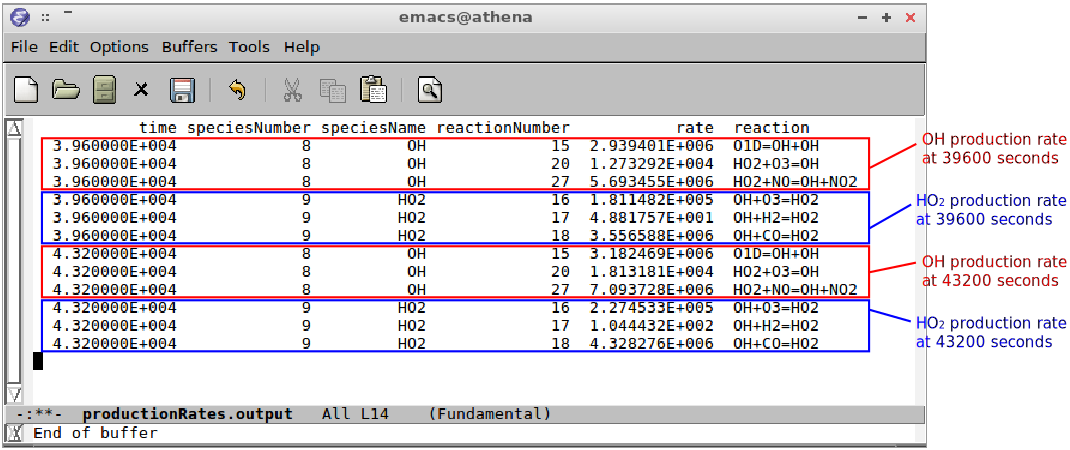
\includegraphics[width=0.95\textwidth]{output-rates.png}
  \caption{Format of the file \texttt{productionRates.output}. The file
    \texttt{lossRates.output} has a similar format.} \label{fig:ropa}
\end{figure}

While the model is running, diagnostic information is printed
to the terminal: this can be redirected to a log file using standard
unix commands. A successfull model run completes with a message
similar to the one shown in Sect.~\ref{sec:install}.

% -----------------------------------------------------------------------------
%
% Copyright (c) 2017 Sam Cox, Roberto Sommariva
%
% This file is part of the AtChem2 software package.
%
% This file is covered by the MIT license which can be found in the file
% LICENSE.md at the top level of the AtChem2 distribution.
%
% -----------------------------------------------------------------------------
\chapter{Model Development} \label{ch:development}

% -------------------------------------------------------------------- %
\section{General Information} \label{sec:information}

Two versions of Atchem2 are available:

\begin{enumerate}
\item the stable version, which is indicated by a version number
  (e.g., \textbf{v1.0}), and can be found
  \href{https://github.com/AtChem/AtChem2/releases}{here}.
\item the development version: which is indicated by a version number
  with the suffix \texttt{-dev} (e.g., \textbf{v1.1-dev}), and can be
  downloaded from the \texttt{master\ branch}
  (https://github.com/AtChem/AtChem2/archive/master.zip) or obtained
  via \textbf{git}.
\end{enumerate}

AtChem2 is under active development, which means that the
\texttt{master\ branch} may sometimes be a few steps ahead of the
latest stable release. The \hyperref[sec:testsuite]{Test Suite} is
designed to ensure that changes to the code do not cause unintended
behaviour or unexplained differences in the model results, so the
development version is usually safe to use, although caution is
advised.

The roadmap for the development of Atchem2 can be found
\href{https://github.com/AtChem/AtChem2/projects/1}{here}.

Feedback, bug reports, comments and suggestions are welcome. Please
check \href{https://github.com/AtChem/AtChem2/issues}{this page} for a
list of known and current issues.

If you want to contribute to the model development, the best way is to
use \textbf{git}. The procedure to contribute code is described
below. A basic level of
\href{https://swcarpentry.github.io/git-novice/}{knowledge of git} is
\emph{required}.

\begin{enumerate}
\item Fork the official repository (\texttt{AtChem/AtChem2}) to your
  github account (\texttt{username/AtChem2}).
\item Configure git so that \texttt{origin} is your fork
  (\texttt{username/AtChem2}) and \texttt{upstream} is the official
  repository (\texttt{AtChem/AtChem2}). The output of \texttt{git\
    remote\ -v} should look like this:

\begin{verbatim}
origin  git@github.com:username/AtChem2.git (fetch)
origin  git@github.com:username/AtChem2.git (push)
upstream    git@github.com:AtChem/AtChem2.git (fetch)
upstream    git@github.com:AtChem/AtChem2.git (push)
\end{verbatim}

\item Create a new branch in your local repository. Make your edits on
  the branch, commit and push. Before committing, it is advised to run
  the \hyperref[sec:testsuite]{Test Suite} locally to verify whether
  the changes could cause any problem.
\item Submit a pull request, together with a brief description of the
  proposed changes. One of the admins will review the edits and
  approve them or ask for additional changes, as appropriate.
\end{enumerate}

Contributions can also be submitted via email or via the
\href{https://github.com/AtChem/AtChem2/issues}{issues page}.

A \hyperref[sec:style]{Style Guide} is available for code
contributions. Note that style and indentation of the code are also
checked by the \hyperref[sec:testsuite]{Test Suite}.

% -------------------------------------------------------------------- %
\section{Test Suite} \label{sec:testsuite}

AtChem2 uses \href{https://travis-ci.org/}{Travis CI} for Continuous
Integration testing. This programming approach ensures changes to the
code do not modify the behaviour and the results of the software in an
unintended fashion.

To begin using CI on code modifications, create a Pull Request on
github from your own fork to \texttt{AtChem/AtChem2} (see
\hyperref[sec:information]{previous section} for instructions on how to
set up \textbf{git}). Once the PR is created, Travis CI will
automatically run build, unit and behaviour tests on 2 architectures
(linux and OSX). Pull requests should only be merged once the Travis
CI has completed with passes on both architectures. This is indicated
by the meassage: ``All checks have passed''.

In order to run the Testsuite on your local machine, call
\texttt{make\ alltest} from the \emph{main directory}. This will run
each of the 3 classes of test in this order:

\begin{itemize}
\item unit tests: checks that small fragments of code generate the
  expected outputs;
\item build test: checks that an example program builds and runs
  successfully;
\item behaviour tests: builds each of a number of test setups in turn,
  and checks that they generate the expected outputs.
\end{itemize}

Each of the test classes outputs the results of their tests to the
terminal screen. To perform just the unit tests, call \texttt{make\
  unittests}. To run just the build and behaviour tests, call
\texttt{make\ tests}.

The CI tester performs the following on each architecture:

\begin{itemize}
\item Install \texttt{gfortran}, \texttt{cvode}, and \texttt{numdiff}
  \begin{itemize}
  \item linux: use \texttt{apt-get} for \texttt{gfortran},
    \texttt{numdiff}, and \texttt{liplapack-dev} (a dependency of
    \texttt{cvode}). Install \texttt{cvode} from source
    (\texttt{apt-get} could also be used to install \texttt{sundials}
    (including \texttt{cvode}), but it doesn't currently hold
    \texttt{cvode\ 2.9}).
  \item OSX: use Homebrew for \texttt{gfortran} and
    \texttt{numdiff}. Install \texttt{cvode} from source.
  \end{itemize}
\item Build and run unit tests. PASS if all unit tests pass.
\item Build and run a single example of AtChem2. PASS if this exits
  with 0.
\item Build and run several other examples of AtChem2, using different
  input files. PASS if no differences from the reference output files
  are found, otherwise FAIL. Every test must pass to allow the full CI
  to PASS.
\end{itemize}

\subsection{Adding new unit tests} \label{subsec:adding-new-unit-tests}

To add new unit tests, do the following:

\begin{itemize}
\item Navigate to \texttt{travis/unit\_tests}. This contains several
  files with the ending \texttt{*\_test.f90}. IF the new test to be
  added fits into an existing test file, edit that file - otherwise,
  make a new file, but it must follow that pattern of
  \texttt{*\_test.f90}. It is suggested that unit tests covering
  functions from the source file \texttt{xFunctions.f90} should be
  named \texttt{x\_test.f90}.
\item The file must contain a module with the same name as the file,
  i.e.~\texttt{*\_test}. It must \texttt{use\ fruit}, and any other
  modules as needed.
\item The module should contain subroutines with the naming scheme
  \texttt{test\_*\textasciitilde{}}. These subroutines must take no
  arguments (and, crucially, not have any brackets for arguments
  either - subroutine \texttt{test\_calc} is correct, but subroutine
  \texttt{test\_calc()} is wrong).
\item Each subroutine should call one or more assert functions
  (usually \texttt{assert\_equals()}, \texttt{assert\_not\_equals()},
  \texttt{assert\_true()} or \texttt{assert\_false()}).  These assert
  functions act as the arbiters of pass or failure - each assert must
  pass for the subroutine to pass, and each subroutine must pass for
  the unit tests to pass.
\item The assert functions have the following syntax:

\begin{verbatim}
call assert_true( a == b , "Test that a and b are equal")
call assert_false( a == b , "Test that a and b are not equal")
call assert_equals( a, b , "Test that a and b are equal")
call assert_not_equals( a, b , "Test that a and b are not equal")
\end{verbatim}

\end{itemize}

It is useful to use the last argument as a \emph{unique} and
\emph{descriptive} test message. If any unit tests fail, then this
will be highlighted in the summary, and the message will be
printed. Unique and descriptive messages enable faster and easier
understanding of which test has failed, and perhaps why.

If these steps are followed, calling \texttt{make\ unittests} is
enough to run all the unit tests, including new ones. To check that
your new tests have indeed been run and passed, check the output
summary - you should see a line associated to each of the
\texttt{test*} subroutines in each file in the unit test suite.

\subsection{Adding new behaviour tests} \label{subsec:adding-new-behaviour-tests}

To add a new behaviour test called \texttt{\$TESTNAME} to the
Testsuite, you should provide the following:

Each input \texttt{\$TESTNAME} should have a subdirectory
\texttt{travis/tests/\$TESTNAME/} containing the following files in
the following structure (\texttt{*} indicates that this file/directory
is optional dependent on the configuration used in the test, while
\texttt{+} indicates that this directory should be populated with the
required files for the constraints declared in file in the
\texttt{model/configuration} directory):

\begin{verbatim}
|- mcm
|  |- photolysis-rates_v3.3.1
|  |- peroxy-radicals_v3.3.1
|- model
|  |- configuration
|  |  |- $TESTNAME.fac
|  |  |- environmentVariables.config
|  |  |- mechanism.reac.cmp
|  |  |- mechanism.prod.cmp
|  |  |- mechanism.species.cmp
|  |  |- mechanism.ro2.cmp
|  |  |- model.parameters
|  |  |- outputSpecies.config
|  |  |- outputRates.config
|  |  |- *photolysisConstant.config
|  |  |- *photolysisConstrained.config
|  |  |- solver.parameters
|  |  |- *speciesConstrained.config
|  |  |- *speciesConstant.config
|  |  |- initialConcentrations.config
|  |  `- a .gitignore file containing
|  |
|  |       # Ignore everything in this directory
|  |       *
|  |       # Except the following
|  |       !*.config
|  |       !*.parameters
|  |       !.gitignore
|  `- constraints
|     |- *+environment (1)
|     |  `- a .gitignore file containing
|     |     # Ignore nothing in this directory
|     |
|     |         # Except this file
|     |         !.gitignore
|     |
|     |- *+photolysis (1)
|     |  `- a .gitignore file containing
|     |             # Ignore nothing in this directory
|     |
|     |         # Except this file
|     |         !.gitignore
|     |
|     `- *+species (1)
|        `- a .gitignore file containing
|               # Ignore nothing in this directory
|
|               # Except this file
|               !.gitignore
|- output
|  |- reactionRates/ (3)
|  |- concentration.output.cmp
|  |- environmentVariables.output.cmp
|  |- errors.output.cmp
|  |- finalModelState.output.cmp
|  |- initialConditionsSetting.output.cmp
|  |- jacobian.output.cmp
|  |- lossRates.output.cmp
|  |- mainSolverParameters.output.cmp
|  |- photolysisRates.output.cmp
|  |- photolysisRatesParameters.output.cmp
|  `- productionRates.output.cmp
|- $TESTNAME.out.cmp (2)
\end{verbatim}

Notes on this structure:

\begin{itemize}
\item if any environment variables (resp. species, photolysis) are to
  be constrained by data from a file (as set in
  \texttt{model/configuration/environmentVariables.config},
  \texttt{model/configuration/speciesConstrained.config},\\
  \texttt{model/configuration/photolysisConstrained.config}), the
  subdirectories in \texttt{model/constraints/}
  (\texttt{environment/}, \texttt{species/}, \texttt{photolysis/})
  should contain data files with filename equal to the constrained
  variable name.
\item the file \texttt{\$TESTNAME.out.cmp}, should contain a copy of
  the expected screen output;
\item the subdirectory \texttt{reactionRates}, should contain a
  \texttt{.gitignore} file and a copy of each of the appropriate files
  normally outputted to \texttt{reactionRates}, with each suffixed by
  \texttt{.cmp}. The \texttt{.gitignore} file should contain

\begin{verbatim}
       \# Ignore everything in this folder
       \*
       \# except files ending in .cmp
       !*.cmp
\end{verbatim}
\end{itemize}

New tests will be picked up by the Makefile automatically when running
\texttt{make\ test}.

% -------------------------------------------------------------------- %
\section{Style Guide} \label{sec:style}

In order to make the code more readable, we attempt to use a
consistent style of coding. Two scripts, \texttt{tools/fix\_style.py}
and \texttt{tools/fix\_indent.py}, help with keeping the style of the
Fortran code consistent:

\begin{itemize}
\item \texttt{tools/fix\_style.py} edits files in-place to try to be
  consistent with the style guide (passing two arguments sends the
  output to the second argument, leaving the input file untouched, and
  is thus the safer option). This script is by no means infallible.;
  therefore, when using the script (by invoking \texttt{python\
    tools/fix\_style.py\ filename}), it is strongly recommended to
  have a
  backup of the file to revert to, in case this script wrongly edits.\\
  This script is also used in the \hyperref[sec:testsuite]{Test Suite}
  to check a few aspects of the styling. This works by running the
  script over the source file and outputting to a \texttt{.cmp} file:
  if the copy matches the original file, then the test passes.
\item \texttt{tools/fix\_indent.py} works similarly, but checks and
  corrects the indentation level of each line of code. This is also
  used within the \hyperref[sec:testsuite]{Test Suite}.
\end{itemize}

\subsection{Style recommendations} \label{subsec:style-recommendations}

\subsubsection{General principles} \label{general-principles}

\begin{itemize}
\item All code should be within a module structure, except the main
  program.  In our case, due to a complicating factor with linking to
  CVODE, we also place \texttt{FCVFUN()} and \texttt{FCVJTIMES()}
  within the main file \texttt{atchem.f90}.
\item Code is write in free-form Fortran, so source files should end
  in \texttt{.f90}
\item Use two spaces to indent blocks
\item Comment each procedure with a high-level explanation of what
  that procedure does.
\item Comment at the top of each file with author, date, purpose of
  code.
\item Anything in comments is not touched by the style guide, although
  common sense rules, and any code within comments should probably
  follow the rules below.
\end{itemize}

\subsubsection{Specific recommendations} \label{specific-recommendations}

\begin{itemize}
\item All \textbf{keywords} are lowercase, e.g.~\texttt{if\ then},
  \texttt{call}, \texttt{module}, \texttt{integer}, \texttt{real},
  \texttt{only}, \texttt{intrinsic}. This also includes
  \texttt{(kind=XX)} and \texttt{(len=XX)} statements.
\item All \textbf{intrinsic} function names are lowercase,
  e.g.~\texttt{trim}, `adjustl', 'adjustr`.
\item \textbf{Relational operators} should use
  \texttt{\textgreater{}=}, \texttt{==} rather than \texttt{.GE.},
  \texttt{.EQ.}, and surrounded by a single space.
\item \texttt{=} should be surrounded by one space when used as
  assignment, except in the cases of \texttt{(kind=XX)} and
  \texttt{(len=XX)} where no spaces should be used.
\item \textbf{Mathematical operators} should be surrounded by one
  space, e.g.~\texttt{*}, \texttt{-}, \texttt{+}, \texttt{**}.
  \begin{itemize}
  \item The case of scientific number notation requires no spaces
    around the \texttt{+} or \texttt{-}, e.g.~\texttt{1.5e-9}.
  \end{itemize}
\item \textbf{Variables} begin with lowercase, while
  \textbf{procedures} (that is, subroutines and functions) begin with
  uppercase. An exception is \textbf{third-party functions}, which
  should be uppercase. Use either CamelCase or underscores to write
  multiple-word identifiers.
\item \textbf{All procedures and modules} should include the `implicit
  none' statement.
\item All variable \textbf{declarations} should include the
  \texttt{::} notation.
\item All procedure dummy arguments should include an \textbf{intent}
  statement in their declaration.
\item \textbf{Brackets}:
  \begin{itemize}
  \item Opening brackets always have no space before them, except for
    \texttt{read}, \texttt{write}, \texttt{open}, \texttt{close}
    statements.
  \item \texttt{call} statements, and the definitions of all
    procedures should contain \textbf{one} space inside the brackets
    before the first argument and after the last argument,
    e.g.~\texttt{call\ function\_name(\ arg1,\ arg2\ )},
    \texttt{subroutine\ subroutine\_name(\ arg1\ )}
  \item Functions calls, and array indices have \textbf{no such space}
    before the first argument or after the last argument.
  \end{itemize}
\end{itemize}

% -----------------------------------------------------------------------------
%
% Copyright (c) 2017 Sam Cox, Roberto Sommariva
%
% This file is part of the AtChem2 software package.
%
% This file is covered by the MIT license which can be found in the file
% LICENSE.md at the top level of the AtChem2 distribution.
%
% -----------------------------------------------------------------------------

\chapter{Credits and Acknowledgements} \label{ch:credits}

% -------------------------------------------------------------------- %
\section{Credits} \label{sec:credits}

AtChem2 has been developed at the \textbf{University of Leicester} by:

\begin{itemize}
\item Sam Cox
\item Roberto Sommariva (also at the \textbf{University of Birmingham})
\end{itemize}

Additional code has been contributed by (in alphabetical order):

\begin{itemize}
\item Maarten Fabr{\'e}
\item Alfred Mayhew
\item Beth Nelson
\item Mike Newland
\item Marios Panagi
\end{itemize}

AtChem2 is a development of\href{https://atchem.leeds.ac.uk/webapp/}{AtChem-online},
created at the \textbf{University of Leeds} by:

\begin{itemize}
\item Chris Martin
\item Kasia Boro{\'n}ska
\item Jenny Young
\item Peter Jimack
\item Mike Pilling
\end{itemize}

Model evaluation and testing of AtChem-online was performed by Andrew
Rickard (NCAS/York) and Monica V{\'a}zquez Moreno (CEAM/EUPHORE), and
technical support was provided by David Waller (University of Leeds).

% ------------------------------------------------------------------- %
\section{Acknowledgements} \label{sec:acknowledgements}

Thanks for their support, feedback, and contributions to (in alphabetical order):

\begin{itemize}
\item Bill Bloss
\item Peter Br{\"a}uer
\item Nahid Chowdhury
\item Vasilis Matthaios
\item Killian Murphy
\item Paul Monks
\item Jon Wakelin
\item Robert Woodward-Massey
\end{itemize}

Many thanks to Harald Stark (University of Colorado-Boulder, USA) for providing
the observational data used to test the photolysis rates subroutines.

% -------------------------------------------------------------------- %
\section{Funding} \label{sec:funding}

Funding provided, at different stages, by:

\begin{itemize}
\item \href{https://www.eurochamp.org}{EUROCHAMP} project.
\item National Centre for Atmospheric Science (\href{https://www.ncas.ac.uk}{NCAS}).
\item Natural Environment Research Council (\href{https://nerc.ukri.org}{NERC}).
\item Met Office (https://www.metoffice.gov.uk).
\item University of Leicester ReSET programme.
\end{itemize}


\bibliographystyle{abbrvnat}
\bibliography{References}
\addcontentsline{toc}{chapter}{References}

\end{document}

%    make more clear that time is always in UTC
%    tidy list of requirements/dependencies
%    rates output and reaction rates output can't be zero in config
